\documentclass[11pt]{article}
\usepackage[margin=1.1in]{geometry}
\usepackage{amsmath, amssymb, amsthm}
\usepackage{graphicx}
\newtheorem{proposition}{Proposition}
\usepackage{booktabs}
\usepackage[hidelinks]{hyperref}
\graphicspath{{../figures/}}

\title{Neural means and kernel corrections for an EMIT\\ atmospheric radiative-transfer emulator}
\author{Yitzchak Shmalo\thanks{Einstein Institute of Mathematics, The Hebrew University of Jerusalem, Jerusalem, Israel. \texttt{yitzchak.shmalo@gmail.com}.}}
\date{September 2026}

\begin{document}
\maketitle

\begin{abstract}
We compare neural networks, exact Mat\'ern kernel regression, and their combinations on a
six-dimensional radiative-transfer table over the 285-band EMIT grid. Across ten random splits
with validation-based selection and 18{,}884 training samples, input-scaled kernels achieve
$0.095\%$ mean relative radiance error, compared with $0.76\%$ for cubic regression and
$0.39\%$ for a neural network. Residual correction reduces the network error to $0.14\%$;
kernels on wider-network features and their convex stacks reach $0.079\%$ and $0.078\%$.
This small stacking gain does not extend to reflectance tails: the wide stack has a larger
95th-percentile inversion error at every split. Learning-curve, output-rank, and width
experiments expose sensitivity to the representation and tuning protocol. We give exact
residual and error-comparison identities and a conditional stability bound for reflectance
inversion, without asserting universal learning rates. Contrasting OCO-2 results delimit the
coupling's scope. The findings concern interpolation of tabulated physics, not validated
operational retrieval.
\end{abstract}

\section{Introduction}

Imaging spectroscopy missions such as EMIT \cite{green}, SBG, and AVIRIS-NG invert measured radiances for
surface and atmospheric quantities, and the inversion loop calls an atmospheric radiative-transfer
model many times per spectrum. At mission data rates the physics code itself (MODTRAN in the
pipelines relevant here \cite{modtran}) is far too slow, so operational retrievals
interpolate precomputed lookup tables, and a body of work replaces table and physics alike with
learned emulators: Gaussian-process surrogates \cite{lamminpaa}, the neural-network MODTRAN
emulator that serves the EMIT mission's operational atmospheric correction \cite{srtmnet,
isofit}, and, recently, physics-guided and multi-fidelity architectures for correction
coefficients \cite{pkan}; network training itself can draw on a growing toolbox of refinements
\cite{bssz, sjk}.
Both families have a record on emulation tasks of this kind: networks learn their own
representations and scale easily to wide spectral outputs \cite{deeponet, fno}, while kernel
and Gaussian-process methods come with exact solves and a strong record both on
operator-learning benchmarks \cite{batlle} and on smooth, low-dimensional regression
\cite{rw}. Which family is preferable for a given emulation problem, and whether they
can be combined so that neither's advantage is given up, are practical questions that the
structure of the data itself should decide.

This paper studies those questions on a tabulated radiative-transfer emulation problem over the
EMIT wavelength grid, using the coupling construction of \cite{nmkc}: train a neural network on standardized output bands as
the mean, correct it with exact Mat\'ern kernel
regressions --- of its residuals on the input space, and of the target on the network's own
learned features --- and let a per-coordinate selection on held-out data choose, coefficient by
coefficient, among the network, the kernels, and the corrected predictors. We ask what
structure the dataset has, which model families that structure favors, and whether the kernel
correction of a neural mean improves on both of its parents here.

The dataset answers the first question quickly (Section~\ref{sec:data}). The input is
six-dimensional, and two coordinates carry most of the variance of the output; the output spectra
are smooth curves whose empirical rank is a few dozen out of 285 bands; and the map from state to
spectrum is smooth enough that cubic polynomial regression already lands near two percent relative
error. In the taxonomy of \cite{nmkc} this is the regime that favors exact kernel methods, in
contrast to emulation problems with higher-dimensional reduced states where representation
learning carries more of the weight. The interest of the comparison is therefore not whether
some exotic architecture wins, but how the familiar families divide the problem between them
when the geometry is easy, and whether the coupling machinery preserves the best of each.

The contribution is a controlled empirical comparison, an analysis of metric-dependent
model rankings, and exact algebraic diagnostics for the fitted constructions; it is not a new
architecture, a universal rate theorem, or a validated operational retrieval system.

Sections~\ref{sec:methods} and \ref{sec:results} give the protocol and the measurements. The
results are these. With every training row in the solve and a length scale per input, the input-scaled
kernel is the strongest raw-input kernel and narrowly leads the width-512 feature kernel
on mean radiance error; its learned metric is consistent with the expected anisotropy. The kernel regression of the network's residuals does what it was built to
do, handing the network the kernel's accuracy on the smooth components, but it is no longer the
lowest row. A per-component convex stack of the heads is, by about one standard deviation across
the ten splits, while per-coordinate selection does not transfer from validation to test. The
reflectance metric has a difficulty of its own, set by the atmospheric absorption windows in
which the transmitted flux approaches zero: there the sensitivity of the inversion to the path
radiance and the two flux components is unbounded, and at exactly zero flux the physical
reflectance is not identifiable at all. We measure what the metric returns for exact inputs and
report reflectance medians together with all-band tails and a finite-perturbation
stability bound. The tails reveal a ranking reversal not visible in the radiance mean.
Section~\ref{sec:scaling} adds what a single training size cannot show: learning curves from
500 rows to the full block, refits at other output ranks, a ladder of network widths, and the two
questions those curves raise --- where the kernel's hyperparameters should be chosen, since the
protocol used here turns out to cost it a measurable amount, and whether its metric can be read off
the data instead of searched for.
Section~\ref{sec:identity} gives the identity behind the residual correction, which separates exact residual identities and error comparisons from unproved
learning-rate interpretations.
Section~\ref{sec:oco2} records where the constructions that win here do not transfer, on the
OCO-2 problem of the companion paper \cite{nmkc}, and Section~\ref{sec:corpora} applies the same
family set to ten further emulation configurations.

\section{Data and protocol}\label{sec:data}

The data are $n = 23{,}313$ tabulated radiative-transfer evaluations. Each
input $x \in \mathbb{R}^6$ collects the atmospheric and viewing state; the coordinate ranges are
consistent with the standard lookup-table axes for imaging-spectroscopy atmospheric correction
\cite{isofit} --- an aerosol optical depth in $[0.05, 1.2]$, a surface elevation in $[-0.5, 6]$ km,
a water-vapor column in $[0.05, 7]$ cm, a relative azimuth in $[0, 180]^\circ$, a solar zenith
angle in $[0, 65]^\circ$, and a view zenith angle within $30^\circ$ of nadir. Each output is a set
of four spectral components on the same 285-point EMIT wavelength grid spanning
381--2493\,nm: path radiance $Y_1$, direct flux $Y_2$, diffuse flux $Y_3$, and spherical albedo
$Y_4$ (Figure~\ref{fig:examples}). The quantities retrieved downstream are the radiance at a
test surface reflectance $\rho$,
\begin{equation}\label{eq:fwd}
L(\rho) \;=\; Y_1 + \rho\,\frac{Y_2 + Y_3}{1 - \rho\, Y_4},
\end{equation}
and the reflectance recovered by inverting \eqref{eq:fwd} with predicted components at the true
radiance,
\begin{equation}\label{eq:inv}
\hat\rho \;=\; \frac{L - \hat Y_1}{\hat Y_2 + \hat Y_3 + \hat Y_4 (L - \hat Y_1)},
\end{equation}
both evaluated at $\rho = 0.7$.

The protocol is the same for every family. The table is split into a test block of 2{,}331
rows and a remaining block of 20{,}982; 2{,}098 of the latter are held out for validation,
leaving 18{,}884 for fitting. The procedure is repeated with seeds 101--110. Standardization
and principal components are fitted only on each split's training rows. Hyperparameters,
checkpoints, coordinatewise selections and combination weights use that split's validation
rows. Each fitted family is then evaluated on that split's test rows. Unless stated otherwise,
tables report the mean and sample standard deviation over the ten splits.

These splits assess interpolation within one fixed lookup table. An earlier exploratory
version consulted a test split of the same table. Redrawing the split does not erase that
information or create an untouched external dataset: rows can reappear across split roles,
and the study's choice of families and subsequent ablations was informed by earlier results.
The repeated-split evidence is therefore descriptive rather than a confirmatory test on ten
independent datasets. The main and wide-pipeline tables have complete individual records;
some secondary ablations are retained only partly at per-seed level, as specified under data
availability. Paired differences on common splits are reported in
Section~\ref{sec:paired-tails}, without treating their SD as a confidence interval.
The same validation rows serve early stopping, tuning and combination, so they are not an
independent calibration sample and support no coverage guarantee. Evaluation at a single
surface reflectance, $\rho=0.7$, does not establish performance for variable surface spectra.

\begin{figure}[t]
\centering
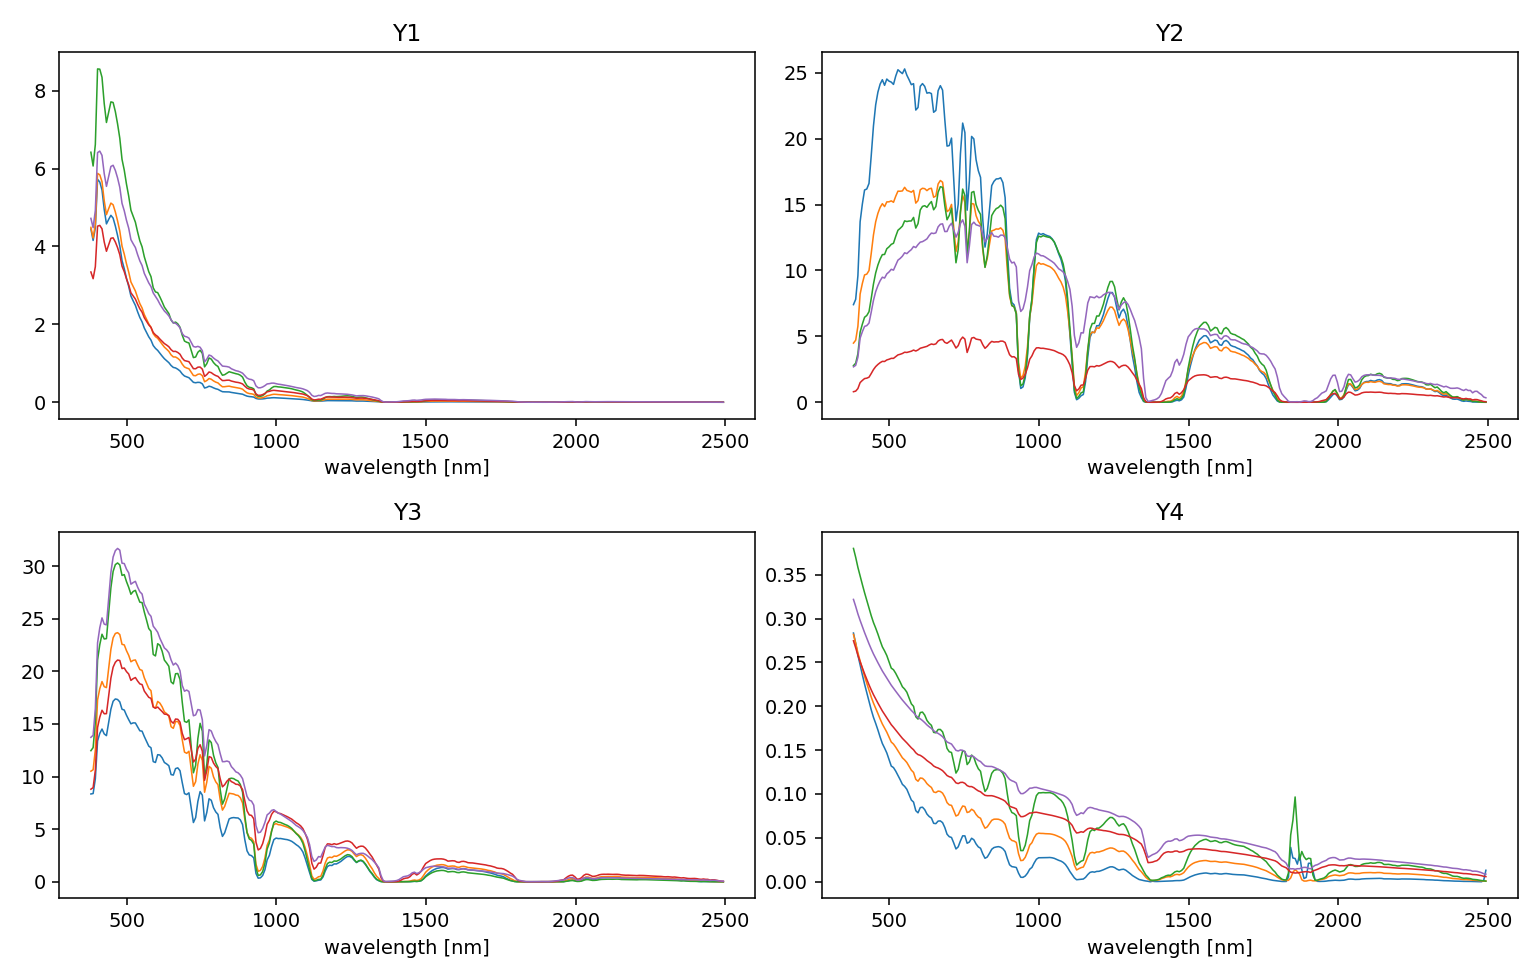
\includegraphics[width=\textwidth]{emit_data_examples.png}
\caption{Example output curves across the EMIT wavelength grid, five samples per panel. The
curves are smooth, share the deep water-vapor absorption features near 1380 and 1900\,nm, and
differ mainly by smooth rescalings along the state axes.}
\label{fig:examples}
\end{figure}

\begin{figure}[t]
\centering
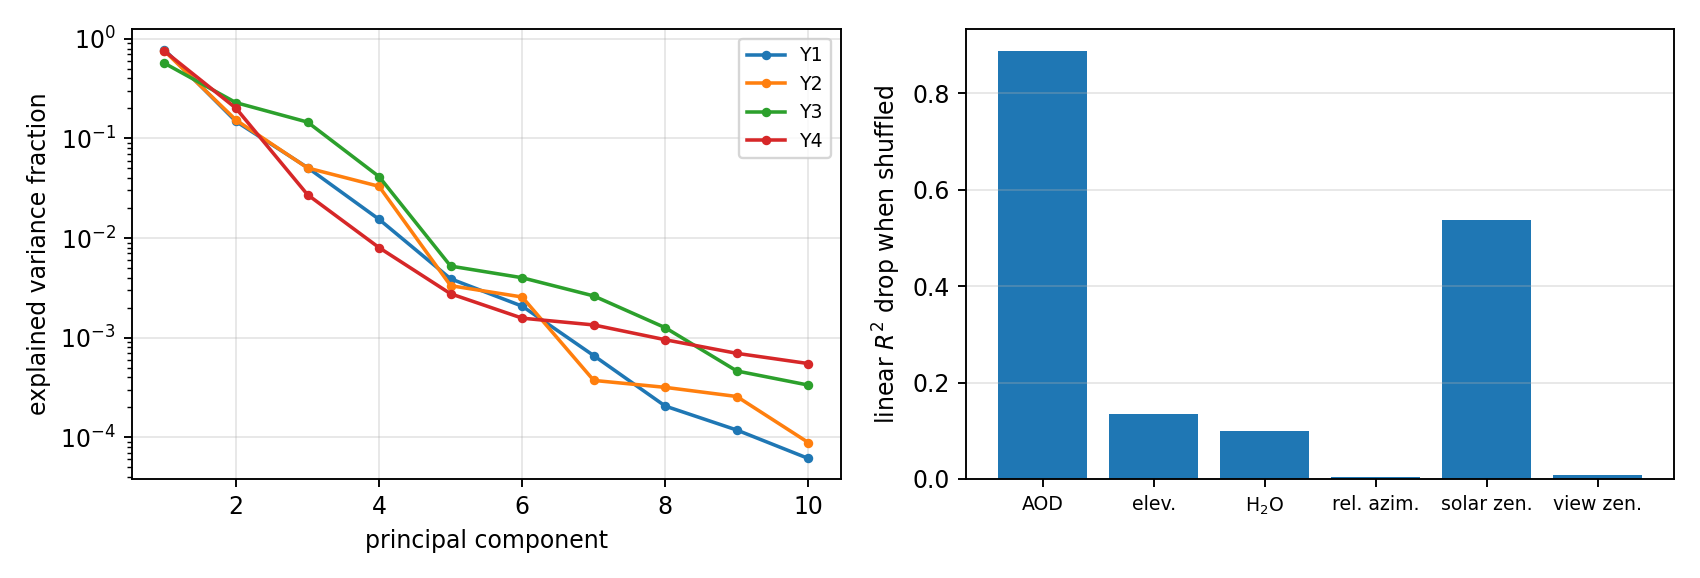
\includegraphics[width=\textwidth]{emit_structure.png}
\caption{Left: explained-variance spectra of the standardized outputs. Every component
concentrates 99.99\% of its variance in 11--25 principal components out of 285 bands. Right:
drop in linear validation $R^2$ when a single standardized input coordinate is shuffled. Aerosol
optical depth and solar zenith angle dominate; the azimuth and view-zenith coordinates are almost
inert at first order.}
\label{fig:structure}
\end{figure}

Three empirical structural diagnostics motivate the model comparison.

\emph{The outputs are low rank.} On standardized training outputs, $99.99\%$ of the variance of
every component lies in the first 11--25 principal components, and $99.9999\%$ in at most 44
(Figure~\ref{fig:structure}, left); the minimum adjacent-band correlation across the four
components is $0.994952$ on the training rows. All regressors below
act on the first 64 principal coefficients, whose training unexplained-variance fraction is
below $10^{-6}$, except the networks, which are trained directly on the 285 standardized
bands. A small aggregate variance tail is not a uniform relative-error guarantee in physical
units; Section~\ref{sec:identity} states the projection error explicitly.

\emph{The measured input relevance is strongly anisotropic.} Shuffling the aerosol coordinate destroys a
linear model's validation $R^2$ (a drop of $0.89$); the solar zenith follows at $0.54$; elevation
and water vapor sit near $0.1$; the two remaining angles barely register
(Figure~\ref{fig:structure}, right). The values reported for these probes, and for the other
structure measurements used to motivate architectures, are their validation-split rescoring;
the initial exploratory versions were test-scored as disclosed above. Six nominal dimensions have four coordinates
with measurable first-order relevance, two of them dominant. This finite-sample diagnostic helps
explain why smooth methods work, but a selected scalar length scale does not remove anisotropy.
Any theorem attributing generalization to anisotropic metric adaptation would also have to
control regularization bias, selection of scale and nugget, and the empirical output-rank
truncation. We use anisotropy as a measured property of this split, not as such a guarantee.

\emph{Low-degree surrogates are accurate.} A linear model in the standardized state reaches $R^2 = 0.83$; distance-weighted
5-nearest-neighbors does worse ($0.74$), so this particular local baseline underperforms the linear one;
and a cubic polynomial ridge reaches mean relative $L^2$ errors near two percent
(Table~\ref{tab:results}). Smooth, low-dimensional, low-rank: in the taxonomy of the companion
paper this is the regime of the Helmholtz and Navier--Stokes benchmarks, where the kernel stage won
the internal selection, not the regime of its OCO-2 problem, where representation learning carried
the problem.

One more property of the task matters for reading any reflectance number. In the deep
absorption windows the transmitted flux $Y_2 + Y_3$ collapses toward zero --- in this table, to
values as small as $10^{-21}$ --- and the inversion \eqref{eq:inv} is undefined at a fully opaque
band ($0/0$): the physical reflectance is non-identifiable there. The protocol maps a non-finite
inverse to zero, but that branch is not what creates the measured true-component error. The
exact components, put through the same evaluation, give a reflectance RMSE of $0.0054$ against
the true $\rho = 0.7$, produced entirely by $0.25\%$ of (sample, band) entries --- $1{,}652$ of
$664{,}620$, measured on the earlier single split, whose test block held one row more than the
ten drawn here --- whose denominators cancel to below $2\times10^{-13}$; every value returned is
finite (the protocol's zero-fill for non-finite inversions is never triggered by the true
components), and the effect is invisible in component errors. What this measures is the
conditioning of the inversion at those entries and not the accuracy of any emulator: it is what
the evaluation returns when the components handed to it are exact. It is not a lower bound on an
emulator's reflectance error. A predictor whose component errors offset the cancellation would
score below it, and a predictor with generic errors of its own can score far above it; what the
measurement establishes is that a mean-square reflectance summary on this table reports the
conditioning of these entries alongside the emulator's errors. Median error summarizes
the center of the distribution but cannot assess its tail; both are reported below.

Differentiating \eqref{eq:inv} separates the components. Write $D = \hat Y_2 + \hat Y_3 +
\hat Y_4 (L - \hat Y_1)$ for its denominator. Then
\begin{equation}\label{eq:sens}
\frac{\partial\hat\rho}{\partial \hat Y_4} = -\hat\rho^{\,2},
\qquad
\frac{\partial\hat\rho}{\partial \hat Y_2} = \frac{\partial\hat\rho}{\partial \hat Y_3}
 = -\frac{\hat\rho}{D},
\qquad
\frac{\partial\hat\rho}{\partial \hat Y_1} = -\frac{\hat Y_2 + \hat Y_3}{D^{2}} .
\end{equation}
At exact, identifiable components, $\widehat\rho=\rho=0.7$ and the albedo derivative is
$-0.49$, independent of the positive transmitted flux. This is a local statement at the
truth, not a global bound for arbitrary predictions: when an inaccurate inverse has large
$|\widehat\rho|$, its albedo derivative can also be large. The explicit inverse-denominator
sensitivity of the path radiance and flux components explains why errors near opaque bands
require separate examination. In the earlier single-split diagnostic, $7.4\%$ of entries had
absolute reflectance error above $0.5$, with $95\%$ of those at flux below one percent of its
median. That earlier diagnostic is not part of the ten-split model comparison. The current
all-band tails are reported directly in Section~\ref{sec:paired-tails}.

\subsection{Finite-perturbation control of the inversion}\label{sec:stability}

The derivatives in \eqref{eq:sens} describe local conditioning. The following elementary
identities give a finite-error test and distinguish forward accuracy from inversion stability.
For one sample and band, write $a=Y_1$, $t=Y_2+Y_3$, $s=Y_4$ and
$L=a+\rho t/(1-\rho s)$. Set
$e_a=\widehat a-a$, $e_t=\widehat t-t$, $e_s=\widehat s-s$.

\begin{proposition}[Conditional radiance and reflectance stability]\label{prop:stability}
Suppose $0\le\rho\le\rho_{\max}$, $t>0$ and $q=1-\rho s>0$. If also
$\widehat q=1-\rho\widehat s>0$, the forward error satisfies the exact identity
\begin{equation}\label{eq:forward-error}
 \widehat L-L=e_a+\frac{\rho e_t}{\widehat q}
                  +\frac{\rho^2 t e_s}{q\widehat q}.
\end{equation}
In particular, if $q,\widehat q\ge\kappa>0$,
\[
 |\widehat L-L|\le |e_a|+\rho_{\max}|e_t|/\kappa
                         +\rho_{\max}^2|t e_s|/\kappa^2.
\]
For inversion at the true radiance, put
$u=L-a=\rho t/q$, $D=t/q$, and
$\widehat D=\widehat t+\widehat s(L-\widehat a)$. Whenever $\widehat D\ne0$,
\begin{equation}\label{eq:inverse-error}
 \widehat\rho-\rho=
 -\frac{(1-\rho\widehat s)e_a+\rho e_t+\rho u e_s}{\widehat D},
 \qquad
 \widehat D-D=e_t+u e_s-\widehat s e_a.
\end{equation}
If
$B=|e_t|+|u e_s|+|\widehat s e_a|\le\eta D$ for some $0\le\eta<1$, then
$\widehat D\ge(1-\eta)D>0$ and
\begin{equation}\label{eq:inverse-bound}
 |\widehat\rho-\rho|\le
 \frac{|1-\rho\widehat s|\,|e_a|+\rho|e_t|+\rho|u e_s|}{(1-\eta)D}.
\end{equation}
\end{proposition}
\begin{proof}
Subtract the two forward maps and use
$1/\widehat q-1/q=\rho e_s/(q\widehat q)$ to obtain
\eqref{eq:forward-error}. Since $u=\rho D$,
$\widehat D=D+e_t+u e_s-\widehat s e_a$ and
$\widehat\rho-\rho=(u-e_a-\rho\widehat D)/\widehat D$, which gives
\eqref{eq:inverse-error}. The triangle inequality yields
$|\widehat D-D|\le B$ and then \eqref{eq:inverse-bound}.
\end{proof}

When $\widehat q\ne0$, the same calculation gives the exact forward--inverse link
\begin{equation}\label{eq:forward-inverse-link}
 \widehat\rho-\rho=-\frac{\widehat q}{\widehat D}(\widehat L-L).
\end{equation}
Consequently, on a common set where $|\widehat q|\le Q$ and
$|\widehat D|\ge\delta>0$, the corresponding unweighted $L^2$ errors obey
$\|\widehat\rho-\rho\|_2\le(Q/\delta)\|\widehat L-L\|_2$.
Without the denominator condition there is no uniform implication from small spectral
relative radiance error to small reflectance error. For example, take two bands with
$a=s=0$, $t=(1,\varepsilon)$ and $0<\rho<1$. A predictor with
$\widehat t=t$, $\widehat s=0$ and $\widehat a=(0,c\varepsilon)$, where $0<c<\rho$,
has relative spectral radiance error
$c\varepsilon/(\rho\sqrt{1+\varepsilon^2})\to0$ but retrieves
$(\rho,\rho-c)$, so its reflectance RMSE remains $c/\sqrt2$. Every denominator is
positive for $\varepsilon>0$ and both retrieved reflectances remain physical. This is a
finite synthetic example, not an additional EMIT experiment.

The forward bound need not deteriorate when $t$ tends to zero, whereas the inverse bound
requires error control relative to $D=t/q$. Thus a small spectral radiance error does not
certify stable reflectance recovery. At $t=0$, $L=a$ is independent of $\rho$ wherever the
forward formula is defined, so reflectance is unidentifiable from this band. The identities
are exact-arithmetic statements; floating-point cancellation in $L-a$ can further affect an
implemented inverse.

A retrieval assessment should therefore specify a common application passband and a
conditioning threshold before comparing predictors, report the retained fraction, and count
invalid inversions instead of hiding them by zero filling or clipping. The utility
\path{code/conditioned_reflectance.py} implements this diagnostic with a threshold relative
to a positive flux scale determined on training data and a common truth-based evaluation mask.
The latter is available in a simulation benchmark, not automatically in a real retrieval.
Prediction failures on that mask are reported separately. This diagnostic is supplied for
reruns with the original arrays; conditioned EMIT results cannot be reconstructed from the
public aggregate metrics and are not claimed here. The all-band tail analysis in
Section~\ref{sec:paired-tails} uses only quantities already stored in the public run records.


\section{Models}\label{sec:methods}

All models are trained per component and evaluated in physical units after undoing the
standardization; unless stated otherwise they regress the 64 leading principal coefficients of
the standardized component, with the training variance criterion and projection
qualification of Section~\ref{sec:data}. Every hyperparameter named below is selected on the validation set
of the seed at hand. Everything runs on CPU.

\paragraph{Reference family.} Cubic polynomial ridge regression, acting on all monomials of
degree at most three in the six standardized inputs, with the ridge weight selected from
$\{10^{-10},\allowbreak 10^{-8},\allowbreak 10^{-6},\allowbreak 10^{-4},\allowbreak 10^{-2}\}$.
It provides a low-cost, low-degree reference; its empirical error alone does not prove
a smoothness class for the underlying function.

\paragraph{Exact kernel ridge regression.} Three constructions, all Mat\'ern kernels on the
standardized inputs with the length scale expressed as a multiple of the median pairwise
distance of the fit set. The listed nugget is $\gamma$ in $(K+n\gamma I)\alpha=Z$, not the unscaled
diagonal term. The first construction is kept for comparison: a Mat\'ern-$5/2$ kernel fitted on a uniformly drawn subset of 4{,}000 training
points, one eigendecomposition per length scale, multiplier in $\{1,2\}$, nugget in
$\{10^{-8},10^{-6},10^{-4},10^{-2}\}$. The second is the exact solve on every training row:
smoothness $\nu\in\{3/2,5/2\}$, multiplier in $\{0.5,1,2,4\}$ and the same nugget grid, tuned on
validation from a 6{,}000-row training subsample and the winner refit on all 18{,}884 rows by one
Cholesky factorization. The third gives each input its own length scale: starting from the
isotropic winner, a coordinate search over per-input multipliers in $\{1/4,1/2,1,2,4\}$, two
sweeps, scored on validation, after which the smoothness, scale and nugget are re-tuned at the
found metric and the solve is refit on every row. The input relevance measured in
Section~\ref{sec:data} spans more than an order of magnitude across the six coordinates, which
is what the third construction is for.

\paragraph{Fully connected networks.} Three ELU hidden layers of 512 units per component,
trained on the 285 standardized bands with AdamW at learning rate $10^{-3}$, cosine decay, batch
size 1024, weight decay $10^{-6}$, up to 150 epochs with early stopping on validation loss
(patience 25). Five networks are trained per component and seed from different initializations;
the table reports the first and the mean of the five.

\paragraph{Kernel corrections of the neural mean.} The construction of \cite{nmkc}, with the
exact stages now fitted on every training row. (i) \emph{Residual correction}: an exact Mat\'ern
regression, on the standardized input space, of the network's training residuals in coefficient
space, added back to the network's projection into that space, with smoothness, scale
and nugget selected by the validation error of the corrected prediction; applied to the single network and to the five-network mean.
(ii) \emph{Kernel on features}: the same exact regression with the input metric replaced by the
network's last hidden layer, standardized, so that the kernel's exactness is spent in
coordinates the network has already straightened. This is the post-hoc counterpart of deep
kernel learning \cite{wilson}, in which the representation and the kernel are trained
together, and of the kernel-flow regularization of a network's inner layers \cite{yoo}; here
the representation is fixed first and the kernel is solved exactly on it. (iii) \emph{Per-coordinate selection}: for
each of the 64 output coefficients independently, pick on validation among the exact kernel, the
network, the ensemble, the two corrected predictors and the feature kernel, and assemble the
test prediction from the winners. (iv) \emph{Convex stack}: per component, a convex combination
of the same six heads with weights fitted on the validation points in the physical relative
metric, in the manner of stacked generalization \cite{wolpert} and stacked regression
\cite{breiman}. The choice of weighting rule for pools of this kind, and its relation to
constrained minimum-variance weighting, is studied separately and is not part of this
comparison.

\paragraph{What is evaluated at other budgets.} Section~\ref{sec:scaling} repeats the isotropic
exact kernel, the network, its residual correction and the feature kernel at nested training
sizes, at other output ranks and at a wider network; the table of Section~\ref{sec:results} is
the full-size, rank-64, width-512 cell of that grid.

\section{Results}\label{sec:results}

\begin{table}[t]
\centering\small

\resizebox{\textwidth}{!}{\begin{tabular}{lcccccc}
\toprule
 & \multicolumn{4}{c}{component rel.\ $L^2$ [\%]} & radiance & reflectance \\
\cmidrule(lr){2-5}
model & $Y_1$ & $Y_2$ & $Y_3$ & $Y_4$ & rel.\ $L^2$ [\%] & med.\ $|\hat\rho-\rho|$ [\%] \\
\midrule
Cubic ridge & 1.16$\pm$0.02 & 2.18$\pm$0.04 & 1.11$\pm$0.03 & 2.98$\pm$0.06 & 0.760$\pm$0.011 & 0.471$\pm$0.010 \\
Mat\'ern KRR, 4000-point fit & 0.17$\pm$0.01 & 0.61$\pm$0.04 & 0.29$\pm$0.02 & 2.44$\pm$0.87 & 0.332$\pm$0.029 & 0.178$\pm$0.030 \\
Mat\'ern KRR, exact on all rows & 0.08$\pm$0.01 & 0.42$\pm$0.03 & 0.20$\pm$0.00 & 2.62$\pm$0.18 & 0.239$\pm$0.016 & 0.141$\pm$0.018 \\
Mat\'ern KRR, per-input scales & 0.08$\pm$0.01 & 0.16$\pm$0.02 & 0.08$\pm$0.01 & 2.18$\pm$0.16 & 0.095$\pm$0.009 & 0.036$\pm$0.004 \\
FC-DNN (3$\times$512) & 0.48$\pm$0.02 & 0.97$\pm$0.04 & 0.41$\pm$0.02 & 3.02$\pm$0.18 & 0.387$\pm$0.012 & 0.245$\pm$0.008 \\
Five-network mean & 0.37$\pm$0.01 & 0.67$\pm$0.03 & 0.28$\pm$0.01 & 2.51$\pm$0.09 & 0.251$\pm$0.006 & 0.163$\pm$0.003 \\
DNN + residual KRR & 0.10$\pm$0.00 & 0.30$\pm$0.02 & 0.16$\pm$0.01 & 2.43$\pm$0.08 & 0.141$\pm$0.006 & 0.089$\pm$0.008 \\
Ensemble + residual KRR & 0.08$\pm$0.00 & 0.27$\pm$0.03 & 0.13$\pm$0.00 & 2.42$\pm$0.17 & 0.123$\pm$0.007 & 0.080$\pm$0.008 \\
Kernel on network features & 0.18$\pm$0.01 & 0.17$\pm$0.01 & 0.10$\pm$0.01 & 1.99$\pm$0.08 & 0.098$\pm$0.007 & 0.054$\pm$0.004 \\
Per-coordinate selection & 0.19$\pm$0.01 & 0.44$\pm$0.10 & 0.13$\pm$0.02 & 2.25$\pm$0.18 & 0.193$\pm$0.022 & 0.123$\pm$0.023 \\
Convex stack & 0.07$\pm$0.00 & 0.16$\pm$0.01 & 0.09$\pm$0.00 & 1.94$\pm$0.06 & 0.087$\pm$0.006 & 0.048$\pm$0.003 \\
\bottomrule
\end{tabular}
}
\caption{Test errors under the protocol of Section~\ref{sec:data}, mean $\pm$ standard deviation
over the ten splits. Component columns are mean relative $L^2$ errors; the radiance column
evaluates \eqref{eq:fwd} at $\rho = 0.7$; the last column is the median absolute reflectance
error of the inversion \eqref{eq:inv}, in reflectance percentage points, under the zero-fill
evaluation of Section~\ref{sec:data}. The median is used because the sensitivity of
\eqref{eq:inv} to the path radiance and the two flux components diverges continuously as the
transmitted flux vanishes, so mean-square and tail-percentile summaries are dominated, for every
model alike, by near-opaque entries; the exact components put through the same evaluation give
an RMSE of about half a percentage point there (Section~\ref{sec:data}), which is a property of
those entries and not a bound on any emulator. The tail summaries are also displayed in Table~\ref{tab:tails}; a small median does
not certify retrieval performance.}
\label{tab:results}
\end{table}

Table~\ref{tab:results} collects the test errors. Every entry is a mean over the ten splits with
its standard deviation, and the spreads are small enough that most of the orderings discussed
below hold seed by seed; where they do not, the text says so.

\paragraph{The scale of the problem.} The cubic ridge reaches $1.86\%$ mean component error and
$0.76\%$ on the radiance: the map is smooth, and a polynomial in six variables recovers it to
two percent. The earlier construction of the kernel regression, a Mat\'ern-$5/2$ on a
4{,}000-point subset, divides both numbers by more than two at seven of the ten splits
($0.74\%$ and $0.31\%$); at the other three its albedo fit collapses ($3.3$--$4.3\%$ against
$1.9\%$), which is what a fit capped at a random subset can do, and its ten-split mean
($0.88\%$, $0.33\%$) carries that fragility.

\paragraph{Exact kernels.} Fitting the same kernel on every training row, one Cholesky
factorization of the $18{,}884\times18{,}884$ Gram matrix per component, lowers the radiance
error to $0.24\%$ and the path-radiance error by half ($0.08\%$ against $0.17\%$), and it has
no collapsing split ($2.3$--$2.9\%$ on the albedo at every seed), but where the capped fit is
sound it is worse on the albedo ($2.6\%$ against $1.9\%$), so the mean component error moves
the wrong way at those splits ($0.83\%$ against $0.74\%$). The albedo is the component whose
principal spectrum decays slowest and whose values sit within a few percent of zero over much of
the grid, and it is also the one where the transfer of a scale and nugget tuned on a 6{,}000-row
subsample to the full solve is least reliable. A length scale per input removes most of this:
the per-input kernel reaches $0.63\%$ on the components and $0.095\%$ on the
radiance, with the best reflectance column of the table ($0.036$ percentage points), and its
albedo column ($2.2\%$) sits between the two isotropic solves. The learned metric is consistent with the expected component anisotropy: for the two flux components and the spherical albedo the coordinate search gives
the relative azimuth a length scale sixteen to thirty-two times longer than the others --- a
median of sixteen on the direct flux and the albedo and of thirty-two on the diffuse flux, at
every one of the ten seeds for the two flux components and at nine of the ten for the albedo,
whose search leaves the azimuth unscaled at the tenth --- and the view zenith two to sixteen
times longer,
while for the path radiance, which
does depend on the viewing geometry, the metric stays nearly isotropic. The weak fitted azimuth dependence is consistent with the physical interpretation of
these components; a finite length-scale search is not a proof of exact invariance. On this table the per-input exact kernel and the kernel on network features (below)
are, within the seed-to-seed spread, the strongest single models.

\paragraph{Networks.} The fully connected network lands at $1.22\%$ and $0.39\%$; the mean of
five independently initialized networks at $0.96\%$ and $0.25\%$, a third off the radiance error
for five times the training cost, the usual decorrelation gain. Neither reaches the isotropic
exact kernel on any of the first three components, and the network's advantage on the albedo
that the single-split study reported does not survive replication: on $Y_4$ the five-network
mean ($2.5\%$) is behind the 4{,}000-point kernel wherever that kernel's fit is sound ($1.9\%$
at seven of the ten seeds) and behind the exact kernel with per-input scales at every seed.

\paragraph{Kernel corrections of the neural mean.} An exact Mat\'ern regression of the
network's residuals on the standardized inputs takes the single network from $0.39\%$ to
$0.14\%$ on the radiance and the five-network mean from $0.25\%$ to $0.12\%$; the kernel fitted
in the network's last-layer features (DKR) reaches $0.61\%$ and $0.098\%$, indistinguishable
from the per-input kernel on the components and on the radiance --- $0.098$ against $0.095$, the
lower at six seeds of ten --- but half again worse on the reflectance median, $0.054$ against
$0.036$ points, and worse there at every one of the ten. The correction therefore does exactly what it did on the single split ---
it hands the network the kernel's accuracy on the smooth components while keeping the network's
own representation --- but with the kernel now allowed its own input metric the corrected
network is no longer the lowest row: the ordering by radiance error is stack, per-input kernel,
DKR, corrected ensemble, corrected network, with the first four within $0.04$ percentage points
of one another.

\paragraph{Selection and stacking.} Both combiners here draw on the same six heads --- the
isotropic exact kernel, the network, the five-network mean, the two corrected predictors and
the feature kernel --- and not on the per-input kernel, which is the strongest single row of
the table. The per-coordinate selection among those six, made on validation, does not
transfer: its test radiance error ($0.19\%$) is worse than three of the heads it selects
among, and its spread over seeds ($\pm0.02$) is among the largest in the table. The per-component convex stack, with weights fitted on the validation rows in the
physical relative metric, is the best aggregate row ($0.57\%$ components, $0.087\%$ radiance,
$0.048$ reflectance points) and wins the path radiance and the albedo columns outright; its gain
over the strongest single row of the table is eight percent on the radiance and ten percent on
the components, of the order of one standard deviation of either; measured against the best
model the stack actually contains, the kernel on network features, it is eleven percent on the
radiance and seven percent on the components. The paired view is sharper than the marginal one: split by split,
the stack beats the per-input kernel on the components in nine of the ten splits
(mean difference $0.06$ points, spread $0.05$) and beats DKR in all ten
($0.047 \pm 0.006$), while the per-input kernel and DKR trade places (six of ten). The
stack is the best row, and the residual correlations among the members it actually contains say
why it can be: on the path radiance the residuals of the isotropic exact kernel and of the
five-network mean are correlated at $0.27 \pm 0.09$, below the ratio of their errors ($0.34$) at
every one of the ten splits, which is the classical admission condition for a combination to
improve on its better member \cite{bates-granger}, in the form used in \cite{nmkc}. This admission diagnostic concerns a quadratic
error metric; it does not directly guarantee improvement in the mean-relative-norm objective
used by this stack or in the nonlinear downstream inverse. Not every pair in the pool admits: the two residual-corrected predictors are correlated at $0.88$ on the
path radiance and at $0.99$ on the albedo, and are largely two views of the same predictor. The observed gain is compatible with complementary errors among the heads. It does not
make every pair useful, and the best albedo head in this pool is the feature kernel, not the
residual-corrected networks. The coordinatewise rule performs worse under this validation
budget; both sampling variability and its different selection objective may contribute.

\paragraph{Comparison with the single-split study.} The earlier version of this study reported
the corrected network as the lowest row, at $0.25\%$ radiance error, and the exact kernel on the
raw state at $0.41\%$; both numbers came from a single split whose test block had been consulted
during exploration and from a kernel fitted on 4{,}000 points with one length scale. Under the
fresh-seed protocol the corrected network reads $0.14\%$ and the exact kernel with per-input
scales $0.095\%$. The smoothness of the map, the complementarity of the heads across components
and the mechanism of the residual correction hold under replication; the claim that the
corrected network is the best model on this table does not.

\paragraph{The albedo.} Every family is worst on $Y_4$ by an order of magnitude, and the
per-band errors show why: the spherical albedo's values in the short-wave infrared are close to
zero, so relative error is large for every model there, and the component is hard for reasons
of signal-to-noise rather than of model class. The stack's $1.94\%$ is the best number any
construction reaches at this training size.

\subsection{Paired comparisons and the radiance--reflectance trade-off}\label{sec:paired-tails}

Paired differences compare two families on the same split. Table~\ref{tab:paired} reports them
for the main and wide pipelines, with positive gains favoring the candidate. The wide feature
kernel improves on the input-scaled kernel at all ten splits, by $0.0165\pm0.0066$ radiance
percentage points. The wide stack's improvement over its own feature kernel is $0.0006\pm0.0026$
points, with eight wins and two losses: small against the split-to-split variation of the
difference itself.

\begin{table}[t]
\centering\small
\resizebox{\textwidth}{!}{\begin{tabular}{lrrr}
\toprule
candidate / reference & mean gain $\pm$ SD [pp] & gain range [pp] & wins/10 \\
\midrule
Input-scaled / isotropic KRR & 0.1436$\pm$0.0122 & [0.1196, 0.1585] & 10 \\
Residual correction / network & 0.2464$\pm$0.0090 & [0.2365, 0.2615] & 10 \\
Narrow stack / input-scaled KRR & 0.0083$\pm$0.0066 & [-0.0054, 0.0185] & 9 \\
Wide feature kernel / input-scaled KRR & 0.0165$\pm$0.0066 & [0.0054, 0.0295] & 10 \\
Wide / narrow feature kernel & 0.0191$\pm$0.0079 & [0.0096, 0.0352] & 10 \\
Wide stack / wide feature kernel & 0.0006$\pm$0.0026 & [-0.0053, 0.0037] & 8 \\
\bottomrule
\end{tabular}
}
\caption{Paired radiance contrasts on seeds 101--110. Gain is the reference error minus the
candidate error, in percentage points (pp). SD is the sample standard deviation of the ten
paired differences; the range and the win count describe the same ten differences.}
\label{tab:paired}
\end{table}

Radiance and reflectance order the families differently. Table~\ref{tab:tails} reports the
all-band reflectance tails beside the medians; each entry averages a within-split statistic, so
the mean of ten 95th percentiles is not a pooled 95th percentile. For the width-512 pipeline the
convex stack lowers the radiance error relative to the feature kernel but raises the mean 95th
percentile of the reflectance error from $7.75$ to $29.44$ points, and the tail is worse at all
ten splits, by factors between $2.63$ and $4.94$. The width-2000 pipeline repeats the reversal:
$7.57$ points for the feature kernel and $22.71$ for the stack, worse at all ten splits by
factors between $2.36$ and $3.79$. The near-tie at $0.079\%$ against $0.078\%$ radiance error
hides a threefold difference in the inverse.

\begin{table}[t]
\centering\small
\resizebox{\textwidth}{!}{\begin{tabular}{lrrrr}
\toprule
model & radiance [\%] & median [pp] & 95th percentile [pp] & RMSE [pp] \\
\midrule
Cubic ridge & 0.760$\pm$0.011 & 0.471$\pm$0.010 & 70.68$\pm$0.02 & 4.18e+03 \\
Isotropic KRR & 0.239$\pm$0.016 & 0.141$\pm$0.018 & 69.53$\pm$0.42 & 4.18e+03 \\
Input-scaled KRR & 0.095$\pm$0.009 & 0.036$\pm$0.004 & 31.16$\pm$6.21 & 1.34e+04 \\
Narrow feature kernel & 0.098$\pm$0.007 & 0.054$\pm$0.004 & 7.75$\pm$1.13 & 1.78e+03 \\
Narrow convex stack & 0.087$\pm$0.006 & 0.048$\pm$0.003 & 29.44$\pm$5.89 & 1.25e+03 \\
Wide feature kernel & 0.079$\pm$0.009 & 0.045$\pm$0.006 & 7.57$\pm$0.95 & 1.40e+03 \\
Wide convex stack & 0.078$\pm$0.011 & 0.043$\pm$0.005 & 22.71$\pm$4.42 & 5.81e+03 \\
\bottomrule
\end{tabular}
}
\caption{All-band retrieval metrics over the ten splits of the main, concatenated-feature and
wide pipelines. Radiance is the mean relative $L^2$ error; the reflectance median, 95th
percentile and RMSE are in percentage points at $\rho=0.7$. The first three columns show mean
$\pm$ sample standard deviation across splits and RMSE its mean. The inverse is neither
clipped nor restricted to the physical domain; every inverse in these runs is finite, and the
RMSE is dominated by large finite values near zeros of the denominator.
Section~\ref{sec:domain} gives the same comparison on the physical domain.}
\label{tab:tails}
\end{table}

The input-scaled kernel shows the same split between center and tail: its median error is only
$0.0365$ points but its mean 95th percentile is $31.16$ points, while the feature kernels have
slightly larger medians and much smaller tails. The kernel on concatenated features has the
smallest tail of all, $5.93$ points. The identities of Section~\ref{sec:stability} tie the
inverse error to the predicted denominator as well as to the forward error, which is why
optimizing a component or radiance error alone need not control the reflectance tail.


\section{Learning curves, output rank and network width}\label{sec:scaling}

Table~\ref{tab:results} is one cell of a larger design: one training size, one output rank, one
network width. This section varies each in turn, at the same ten seeds, with the same
validation-based selection and one test read per family, for the isotropic exact kernel, the
network, its residual correction and the kernel on its features; the cubic ridge is carried as the
smoothness reference. The per-input kernel and the ensembles are run at full size only.

\begin{table}[t]
\centering\small

\resizebox{\textwidth}{!}{\begin{tabular}{lrcccccc}
\toprule
training rows & seeds & Cubic ridge & KRR, isotropic & KRR, per-input & FC-DNN & DNN + residual KRR & kernel on features \\
\midrule
500 & 10 & 0.846$\pm$0.031 & 0.639$\pm$0.022 & 0.415$\pm$0.024 & 1.961$\pm$0.057 & 0.815$\pm$0.035 & 0.456$\pm$0.020 \\
1,000 & 10 & 0.802$\pm$0.024 & 0.519$\pm$0.034 & 0.260$\pm$0.066 & 1.862$\pm$0.015 & 0.590$\pm$0.027 & 0.316$\pm$0.040 \\
2,000 & 10 & 0.780$\pm$0.016 & 0.424$\pm$0.051 & 0.217$\pm$0.052 & 1.232$\pm$0.034 & 0.376$\pm$0.041 & 0.240$\pm$0.049 \\
4,000 & 10 & 0.769$\pm$0.010 & 0.328$\pm$0.028 & 0.154$\pm$0.037 & 0.830$\pm$0.019 & 0.256$\pm$0.021 & 0.164$\pm$0.033 \\
8,000 & 10 & 0.763$\pm$0.010 & 0.279$\pm$0.020 & 0.119$\pm$0.027 & 0.584$\pm$0.020 & 0.190$\pm$0.014 & 0.121$\pm$0.017 \\
18,884 & 10 & 0.760$\pm$0.011 & 0.239$\pm$0.016 & 0.095$\pm$0.009 & 0.387$\pm$0.012 & 0.141$\pm$0.006 & 0.098$\pm$0.007 \\
\bottomrule
\end{tabular}
}
\caption{Learning curves: radiance relative $L^2$ error [\%] against the number of training rows,
mean $\pm$ standard deviation over the ten splits reported in the archived aggregate.
At $n=8{,}000$, one individual record per kernel campaign is absent from the public archive;
the aggregate values are preserved rather than recomputed from nine records. Each rung uses the first $n$ rows of the seed's
training block; the validation and test blocks are those of Table~\ref{tab:results}, so the top
rung is that table. The per-input kernel repeats its coordinate search at every rung. Component
columns are in Figure~\ref{fig:curves} and in the per-seed records.}
\label{tab:curves}
\end{table}

\begin{figure}[t]
\centering
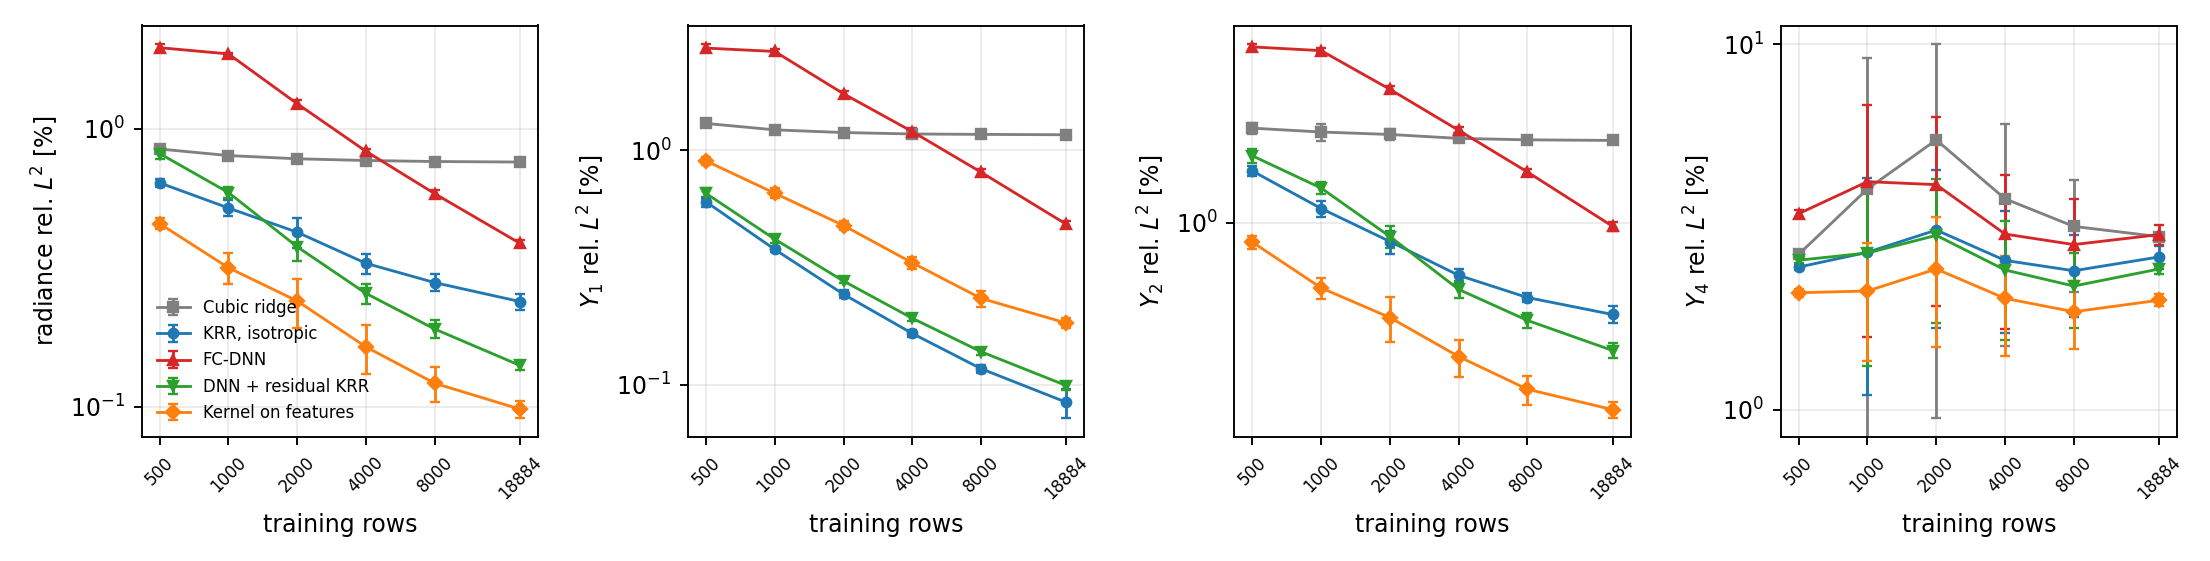
\includegraphics[width=\textwidth]{emit_curves.png}
\caption{Learning curves on log--log axes for the radiance and for three of the four components,
mean and standard deviation over ten splits. The cubic ridge is flat from the first rung; the
kernel, the network, the corrected network and the feature kernel fall at close to $n^{-1/2}$ on
the smooth components and not at all on the spherical albedo. The albedo's spread at $1{,}000$
and $2{,}000$ rows comes from single splits whose albedo fit collapses, the failure
Section~\ref{sec:results} describes for a kernel capped at a random subset; the medians across
splits are flat.}
\label{fig:curves}
\end{figure}

\paragraph{Learning curves.} Each rung uses the first $n$ rows of the seed's training block,
$n = 500$, $1{,}000$, $2{,}000$, $4{,}000$, $8{,}000$ and the full $18{,}884$, with the
validation and test blocks unchanged, so the rungs of one seed are nested and the full
block is the top rung (Table~\ref{tab:curves}, Figure~\ref{fig:curves}).
Three things are visible. First, the cubic is flat: from $0.85\%$ to $0.76\%$ over a factor of
38 in data, a bias floor reached by a thousand rows. Second, on the three smooth components every
other family decays at close to $n^{-1/2}$ (Table~\ref{tab:slopes}): the least-squares slopes of
$\log$ error against $\log n$ over the six rungs lie between $-0.38$ and $-0.61$ for the kernel,
the network, the corrected network and the feature kernel on $Y_1$, $Y_2$ and $Y_3$, while on the
albedo every slope lies between $-0.09$ and $+0.01$: the albedo shows no sustained decrease over this budget range. This plateau does not
distinguish approximation bias, optimization, relative-error weighting or limitations of the
training data.

\begin{table}[t]
\centering\small
\resizebox{\textwidth}{!}{\begin{tabular}{lccccc|ccccc}
\toprule
 & \multicolumn{5}{c|}{slope over the six rungs} & \multicolumn{5}{c}{slope of the last step} \\
family & $Y_1$ & $Y_2$ & $Y_3$ & $Y_4$ & radiance & $Y_1$ & $Y_2$ & $Y_3$ & $Y_4$ & radiance \\
\midrule
Cubic ridge & $-0.03$ & $-0.03$ & $-0.03$ & $-0.02$ & $-0.03$ & $-0.00$ & $-0.01$ & $-0.00$ & $-0.08$ & $-0.01$ \\
KRR, isotropic & $-0.55$ & $-0.38$ & $-0.40$ & $-0.01$ & $-0.28$ & $-0.38$ & $-0.19$ & $-0.17$ & $0.10$ & $-0.18$ \\
KRR, per-input & $-0.45$ & $-0.43$ & $-0.43$ & $0.01$ & $-0.40$ & $-0.32$ & $-0.26$ & $-0.29$ & $0.12$ & $-0.26$ \\
FC-DNN & $-0.50$ & $-0.49$ & $-0.57$ & $-0.09$ & $-0.48$ & $-0.59$ & $-0.60$ & $-0.55$ & $0.07$ & $-0.48$ \\
DNN + residual KRR & $-0.52$ & $-0.53$ & $-0.61$ & $-0.04$ & $-0.50$ & $-0.39$ & $-0.33$ & $-0.39$ & $0.12$ & $-0.35$ \\
Kernel on features & $-0.45$ & $-0.44$ & $-0.46$ & $-0.03$ & $-0.43$ & $-0.28$ & $-0.22$ & $-0.31$ & $0.08$ & $-0.25$ \\
\bottomrule
\end{tabular}
}
\caption{Learning-curve exponents: the least-squares slope of $\log$ error against $\log n$ over
the six rungs of Table~\ref{tab:curves}, and the slope of the last step alone, from $8{,}000$ to
$18{,}884$ rows, per family and component.}
\label{tab:slopes}
\end{table}
These are slopes of six mean errors over a finite sample-size range, not established
asymptotic rates. Standard Sobolev or kernel regression rate formulas require sampling,
source and regularization assumptions \cite{cdv,fs}; neither those assumptions nor the
smoothness norm of the fitted network residual is verified by this experiment.
Third, the kernel's curve bends at the top. Its slope over the
first five rungs is $-0.59$, $-0.44$ and $-0.47$ on the smooth components, and its last step,
from $8{,}000$ to $18{,}884$ rows, is $-0.38$, $-0.19$ and $-0.17$, while the network's last step
is as steep as its average ($-0.59$, $-0.60$ and $-0.55$; Table~\ref{tab:slopes}). Part of this is the tuning protocol:
the kernel's smoothness, scale and nugget are chosen on a $6{,}000$-row subsample at every rung,
so above $6{,}000$ rows the hyperparameters are those of a smaller problem, and
Section~\ref{sec:retune} measures what tuning with every row in the solve recovers: all of it on
the radiance, most of it on the components. The
consequence for the comparison is that the ratio of the network's radiance error to the kernel's
falls from $3.1$ at $500$ rows to $1.6$ at the full block, or to $1.8$ with the kernel tuned on
every row. The kernel's margin over the network
on this table is a margin at this training size; whether it would survive ten times the data
depends on where the kernel's curve settles, which the bend leaves open.

Fourth, and this is the one a single training size cannot show: against the isotropic kernel the
per-input metric changes the measured finite-range slope as well as the error level. Its coordinate search, repeated at every rung,
gives a slope of $-0.399$ on the radiance against the isotropic kernel's $-0.279$, and the ratio
between them falls from $0.65$ at $500$ rows to $0.40$ at the full block, with one step against
that direction ($0.50$ at $1{,}000$ rows, $0.51$ at $2{,}000$) and a fall at every other. The observed discount increases over this sample-size range. The selected metric,
smoothness and nugget all change with sample size, so these measurements do not isolate a
change of asymptotic dimension or establish a faster universal rate. Against the kernel on
network features the margin closes as the data grows. The per-input metric has the lower mean at
all six rungs, but the split-by-split count runs $10$, $9$, $10$, $7$, $5$ and $6$ wins of ten
from $500$ rows to the full block, and the gap itself narrows from $0.415$ against $0.456$ at
$500$ rows to $0.095$ against $0.098$ at the top; the feature kernel's own slope, $-0.435$, is the
steeper of the two. A metric searched on six validated numbers is the better buy on small data,
and a representation learned from the data catches it up. On the albedo the
per-input slope is $+0.01$: the one component no metric rescues.

The corrected network is below both of its parents on the radiance at every one of the ten
splits from $2{,}000$ rows on, and at no split at $500$ or $1{,}000$ rows, where its error sits
between the network's and the kernel's. On $Y_2$ and $Y_3$ it is below both at every split at the
two largest sizes; on $Y_1$ it never is, the isotropic kernel alone being the better head at every
size ($0.084\%$ against $0.099\%$ at the full block). Its exponent is close to the network's and
its error level is closer to the kernel's in these runs. Section~\ref{sec:identity}
gives the exact residual decomposition, while distinguishing it from a proof of these
empirical slopes or of the component-specific exception.

\begin{table}[t]
\centering\small

\resizebox{\textwidth}{!}{\begin{tabular}{lcccccc}
\toprule
PCA rank & variance outside the basis & KRR, isotropic & FC-DNN & DNN + residual KRR & kernel on features \\
\midrule
16 & $7.5\times10^{-4}$ & 0.270$\pm$0.015 & 0.390$\pm$0.015 & 0.175$\pm$0.007 & 0.148$\pm$0.009 \\
32 & $1.5\times10^{-5}$ & 0.243$\pm$0.018 & 0.390$\pm$0.015 & 0.139$\pm$0.006 & 0.102$\pm$0.009 \\
64 & $8.2\times10^{-8}$ & 0.242$\pm$0.018 & 0.390$\pm$0.015 & 0.143$\pm$0.006 & 0.100$\pm$0.009 \\
128 & $5.4\times10^{-9}$ & 0.242$\pm$0.018 & 0.390$\pm$0.015 & 0.150$\pm$0.005 & 0.100$\pm$0.009 \\
285 & $0$ & 0.242$\pm$0.018 & 0.390$\pm$0.015 & 0.172$\pm$0.004 & 0.100$\pm$0.009 \\
\bottomrule
\end{tabular}
}
\caption{Output-rank ablation: radiance relative $L^2$ error [\%] when the kernels and corrections
regress the leading $r$ principal coefficients, mean $\pm$ standard deviation over five splits.
The second column is the fraction of the standardized variance the basis leaves out for the
slowest-decaying component, the spherical albedo; at rank 285 it is zero. The network regresses
the 285 bands directly and is the same predictor in every row.}
\label{tab:rank}
\end{table}

\paragraph{Output rank.} The kernels and corrections regress the leading $r$ principal
coefficients of the standardized component; the network regresses the 285 bands and is the same
predictor at every rank. Table~\ref{tab:rank} refits at $r = 16$, $32$, $128$ and $285$ at five of
the seeds beside the rank-64 rows of those seeds. The kernel is indifferent to the rank above
32: its radiance error reads $0.243$, $0.242$, $0.242$ and $0.242$ at $32$, $64$, $128$ and $285$,
and $0.270$ at $16$, where the truncation leaves $7.5\times10^{-4}$ of the albedo's variance
outside the basis. The kernel on features behaves the same way. The residual correction does not:
it is best at $32$ ($0.139$), a little worse at $64$ ($0.143$), and worse again at $128$ and $285$
($0.150$ and $0.172$). The difference is in what the two regressions fit. The kernel regresses
the component itself, whose tail coefficients are small and smooth functions of the state, and
including them changes these measured errors little; it still has a computational cost. The correction regresses the network's residual, whose tail
coefficients are the network's own errors along directions that hold $10^{-6}$ of the variance,
and a kernel regression of those directions adds a term the $2{,}098$ validation rows select
but the test block does not reward. A rank at the point where the retained variance stops moving,
32 to 64 on this table, is the right setting for the correction, and the rank-64 setting of
Table~\ref{tab:results} is on the safe side of it.

\begin{table}[t]
\centering\small
\resizebox{\textwidth}{!}{\begin{tabular}{llcccccc}
\toprule
 & & \multicolumn{4}{c}{component rel.\ $L^2$ [\%]} & radiance & reflectance \\
\cmidrule(lr){3-6}
network & head & $Y_1$ & $Y_2$ & $Y_3$ & $Y_4$ & rel.\ $L^2$ [\%] & med.\ $|\hat\rho-\rho|$ [\%] \\
\midrule
3$\times$512 & network & 0.48$\pm$0.02 & 0.97$\pm$0.04 & 0.41$\pm$0.02 & 3.02$\pm$0.18 & 0.387$\pm$0.012 & 0.245$\pm$0.008 \\
 & network + residual KRR & 0.10$\pm$0.00 & 0.30$\pm$0.02 & 0.16$\pm$0.01 & 2.43$\pm$0.08 & 0.141$\pm$0.006 & 0.089$\pm$0.008 \\
 & kernel on its features & 0.18$\pm$0.01 & 0.17$\pm$0.01 & 0.10$\pm$0.01 & 1.99$\pm$0.08 & 0.098$\pm$0.007 & 0.054$\pm$0.004 \\
 & per-coordinate selection & 0.19$\pm$0.01 & 0.44$\pm$0.10 & 0.13$\pm$0.02 & 2.25$\pm$0.18 & 0.193$\pm$0.022 & 0.123$\pm$0.023 \\
 & convex stack & 0.07$\pm$0.00 & 0.16$\pm$0.01 & 0.09$\pm$0.00 & 1.94$\pm$0.06 & 0.087$\pm$0.006 & 0.048$\pm$0.003 \\
\midrule
3$\times$2000 & network & 0.93$\pm$0.20 & 2.11$\pm$0.49 & 0.76$\pm$0.19 & 3.27$\pm$0.19 & 0.748$\pm$0.116 & 0.508$\pm$0.110 \\
 & network + residual KRR & 0.12$\pm$0.01 & 0.35$\pm$0.03 & 0.19$\pm$0.03 & 2.35$\pm$0.13 & 0.160$\pm$0.016 & 0.106$\pm$0.010 \\
 & kernel on its features & 0.13$\pm$0.02 & 0.13$\pm$0.02 & 0.08$\pm$0.01 & 2.10$\pm$0.34 & 0.079$\pm$0.009 & 0.045$\pm$0.006 \\
 & per-coordinate selection & 0.14$\pm$0.02 & 0.30$\pm$0.26 & 0.09$\pm$0.01 & 2.55$\pm$0.26 & 0.187$\pm$0.057 & 0.099$\pm$0.033 \\
 & convex stack & 0.08$\pm$0.01 & 0.13$\pm$0.02 & 0.08$\pm$0.00 & 2.00$\pm$0.24 & 0.078$\pm$0.011 & 0.043$\pm$0.005 \\
\bottomrule
\end{tabular}
}
\caption{The pipeline of Section~\ref{sec:methods} run with a $3\times2000$ network in place of
the $3\times512$ one, at the same ten splits: the network (one member, up to 500 epochs under the
same optimizer, learning rate and early stopping), its residual correction, the exact kernel on
its last-layer features, and the per-coordinate selection and convex stack over the wide
pipeline's heads (the isotropic kernel, the network, its correction and its feature kernel),
beside the corresponding rows of Table~\ref{tab:results}; mean $\pm$ standard deviation over the
ten splits.}
\label{tab:wide}
\end{table}

\paragraph{A wider network.} A network of three hidden layers of $2{,}000$ units, trained for up
to 500 epochs under the same optimizer, learning rate and early stopping as the $512$-unit network,
was run at all ten seeds with the rest of the pipeline built on it (Table~\ref{tab:wide}). It is
a worse emulator at every seed, $0.75\%$ against $0.39\%$ on the radiance, and its early stopping
fired between $42$ and $210$ epochs of the $500$ allowed: at this learning rate and batch size this particular wider-network training configuration gives worse standalone predictions.
Width and epoch budget change together; these results do not rule out a better-optimized
wide network. Its representation is better. The exact
kernel on its last-layer features reaches $0.079\%$ on the radiance against $0.098\%$ on the
$512$-unit features, below the per-input kernel's $0.095\%$ at all ten seeds and below the convex
stack of Table~\ref{tab:results} at nine of them, and on the two flux components, at $0.13\%$ and
$0.08\%$, it is at or below every row of that table. The convex stack over the wide pipeline's
heads, which puts $0.88$ to $0.96$ of its weight on that feature kernel, has the lowest mean radiance error in the ten-split comparison at $0.078\%$ on the radiance and $0.043$ reflectance points, below the stack of
Table~\ref{tab:results} at nine of the ten seeds; the per-coordinate selection over the same
heads does not transfer here either. The residual correction of the wider network is a little
worse than that of the narrower one, although that ordering is not guaranteed merely because its base network is worse
(Section~\ref{sec:identity}). A $3\times1000$ rung at the same ten seeds sits between the
two: the network at $0.72\%$, the kernel on its features at $0.088\%$ against $0.098\%$ at
width $512$ and $0.079\%$ at width $2{,}000$. From $512$ to $2{,}000$ the network's own
error rises with width while the error of a kernel on its features falls: what a wider
network learns on this table is a better coordinate system, not a better map. At $4{,}000$
units, run at two seeds, the network is worse again at $0.95\%$ and the kernel on its
features turns back up to $0.097\%$, so the gain in the representation does not continue
past $2{,}000$.

If that reading is right, several networks should give a better coordinate system than one. A
three-member version of the same wide pipeline, run at three seeds, lets the exact kernel see the
concatenated last-layer features of all three members at once, $6{,}000$ coordinates rather than
$2{,}000$. It reads $0.074\%$ on the radiance against $0.083\%$ for the kernel on a single member's
features in the same lanes, lower at all three seeds, and $0.043$ against $0.051$ reflectance
points, again at all three. That puts one exact solve level on the radiance with the convex stack of
six heads fitted in those same lanes ($0.074\%$ against $0.074\%$ on the mean, though the stack is
the lower at two of the three seeds and on the reflectance median at all three). A combination of
six predictors and a single kernel in a wider feature space buy about the same thing here, which is consistent with a useful role for representation diversity. The comparison does not
isolate all optimization and kernel-selection effects. Three seeds provide exploratory evidence rather than a ten-split replication, and the
construction is not run at the width of Table~\ref{tab:results}, so whether the same gain
survives there is left open.

\subsection{Tuning with every row in the solve, and a metric read off the data}\label{sec:retune}

Two further constructions test the two readings above: that the bend at the top of the kernel's
curve is its tuning protocol, and that the metric the coordinate search finds is the physics of
the components. Both were run at all ten seeds (Table~\ref{tab:retune}).

\begin{table}[t]
\centering\small
\resizebox{\textwidth}{!}{\begin{tabular}{lcccccc}
\toprule
 & \multicolumn{4}{c}{component rel.\ $L^2$ [\%]} & radiance & reflectance \\
\cmidrule(lr){2-5}
kernel & $Y_1$ & $Y_2$ & $Y_3$ & $Y_4$ & rel.\ $L^2$ [\%] & med.\ $|\hat\rho-\rho|$ [\%] \\
\midrule
isotropic, tuned on 6{,}000 rows & 0.08$\pm$0.01 & 0.42$\pm$0.03 & 0.20$\pm$0.00 & 2.62$\pm$0.18 & 0.239$\pm$0.016 & 0.141$\pm$0.018 \\
isotropic, tuned on every row & 0.08$\pm$0.00 & 0.36$\pm$0.02 & 0.17$\pm$0.01 & 2.58$\pm$0.14 & 0.210$\pm$0.008 & 0.107$\pm$0.006 \\
per-input search, tuned on 6{,}000 rows & 0.08$\pm$0.01 & 0.16$\pm$0.02 & 0.08$\pm$0.01 & 2.18$\pm$0.16 & 0.095$\pm$0.009 & 0.036$\pm$0.004 \\
per-input search, re-tuned on every row & 0.08$\pm$0.00 & 0.16$\pm$0.02 & 0.08$\pm$0.01 & 2.09$\pm$0.12 & 0.096$\pm$0.009 & 0.036$\pm$0.004 \\
per-input from the cubic's gradients, $p=1$ & 0.34$\pm$0.01 & 0.19$\pm$0.02 & 0.14$\pm$0.01 & 2.17$\pm$0.14 & 0.159$\pm$0.007 & 0.078$\pm$0.004 \\
per-input from the cubic's gradients, $p=1/2$ & 0.11$\pm$0.00 & 0.19$\pm$0.02 & 0.09$\pm$0.01 & 2.27$\pm$0.15 & 0.125$\pm$0.008 & 0.055$\pm$0.004 \\
per-input from the cubic's gradients, $p=1/4$ & 0.08$\pm$0.00 & 0.25$\pm$0.02 & 0.14$\pm$0.01 & 2.38$\pm$0.20 & 0.157$\pm$0.015 & 0.077$\pm$0.013 \\
\bottomrule
\end{tabular}
}
\caption{Where the kernel's hyperparameters are chosen, and how its metric is obtained, at the
full training block and the same ten splits. The first pair tunes smoothness, scale and nugget
on a $6{,}000$-row subsample and on every training row; the last three rows replace the coordinate
search by a metric read off the cubic surrogate's gradients, at three exponents. Selecting the
exponent on validation, per seed, chooses $p=1/2$ at all ten, so that row would duplicate the
$p=1/2$ row and is not printed; the per-seed choices are in the stored numbers. Mean $\pm$ standard
deviation over the ten splits.}
\label{tab:retune}
\end{table}

\paragraph{Tuning with every row in the solve.} The kernel families of
Section~\ref{sec:methods} choose smoothness, scale and nugget by the validation error of a solve
on a $6{,}000$-row subsample, and refit the winner on all $18{,}884$ rows. Doing the tuning
solve on every row instead lowers the isotropic kernel's radiance error from $0.239\%$ to
$0.210\%$ and its reflectance median from $0.141$ to $0.107$ points, better at nine of the ten
splits, the ratio averaging $0.882$ and never above $1.001$. The mechanism is visible in the
chosen scales: over the forty component-seed cells the full block picks a shorter length scale than
the subsample in $26$, the same in $12$, and a longer one in $2$. A tuning set a third of the size
of the solve supports a longer length scale than the solve does, so the subsample protocol
over-smooths, and it over-smooths more the larger the gap between the two.

That is the bend. Below $6{,}000$ rows the tuning subsample \emph{is} the whole training block and
the rungs are already full-block tuned; at $8{,}000$ rows it is three quarters of it; only the top
rung is a third. Applying the measured ratio to the top rung of Table~\ref{tab:curves} takes the
kernel's last step on the radiance from $-0.183$ to $-0.334$, against a slope of $-0.305$ over the
five lower rungs: the top-step slope becomes closer to that of the lower rungs. One retuned endpoint
does not establish a power law over or beyond the observed range. On the two flux components the same correction takes the
last step from $-0.187$ and $-0.171$ to $-0.352$ and $-0.358$ against averages of $-0.437$ and
$-0.468$, so there most of the bend is the protocol and a little of it is not. The consequence for
the comparison of Section~\ref{sec:results} is that the kernel's margin over the network at the
full block is wider than Table~\ref{tab:curves} shows: $1.8$ times rather than $1.6$, under this retuned endpoint. No conclusion about unobserved sample sizes follows.

The same re-tuning does nothing for the per-input kernel: $0.096\%$ against $0.095\%$, better at
four of the ten splits, ratio $1.005$. Its coordinate search already selects a scale of once the
median distance at the metric it finds, which is what the full-block tune selects too. Rescaling
the coordinates removes the over-smoothing that the isotropic kernel suffers, so the per-input
kernel of Table~\ref{tab:results} was never paying the tuning cost, and its number stands as
reported.

\paragraph{A metric read off the data.} The coordinate search costs a sweep over the six inputs at
five multipliers, twice, per component and per seed. The alternative sets the metric before any
kernel is fitted: the multiplier of coordinate $j$ is the root-mean-square gradient of the fitted
cubic surrogate along $j$ over the training rows, raised to a power $p$, normalized to geometric
mean one and clipped to the search's own range $[1/16, 4]$, so a coordinate the map barely responds
to gets a long length scale and $p$ sets how hard the metric leans on that reading. It costs one
cubic fit and six finite differences.

Taken proportionally, at $p=1$, it captures rather more than half the gap: on the radiance it reads
$0.159\%$, below the isotropic kernel at every one of the ten splits by a factor $0.669$ on average
and above the searched metric at every one of them by a factor $1.680$. But $p$ is a free number,
and the ladder is not monotone. The square root reads $0.125\%$ and the fourth root $0.157\%$, so
the best exponent is interior, and choosing it the way every other hyperparameter in this study is
chosen --- the lowest mean validation error over the four components, per seed, with the test block
untouched --- selects $p=1/2$ at all ten seeds. At that exponent the metric closes $79\%$ of the
distance from the isotropic kernel to the searched one on the radiance and $82\%$ on the
reflectance median, for one cubic fit, six finite differences and a choice among three numbers.

The per-band reading says why the exponent matters and what the search still buys. The four
components do not want the same one: $Y_2$ and $Y_3$ are best at $1/2$, the albedo at $1$
($2.18\%$ against $2.27\%$), and the path radiance at $1/4$. $Y_1$ is where the damage is, and it
is worth seeing why. On that component the isotropic kernel already reads $0.084\%$ and the
searched metric $0.085\%$: there is no anisotropy to find. The proportional metric nonetheless
reads $0.34\%$ there, four times worse than doing nothing, because the surrogate's gradient along a
coordinate measures how fast the map moves with it and not how much predictive information it
carries, and on the one component that depends on the viewing geometry those two disagree. Softening
the exponent to $1/4$ takes $Y_1$ back to $0.085\%$, exactly the searched metric's value, at the
cost of $Y_2$ and $Y_3$. So a metric read from first-order sensitivity, with its exponent validated
like any other hyperparameter, is most of what the coordinate search buys at a small fraction of its
cost. What the search still buys is the freedom to be anisotropic differently for each component,
which one global exponent cannot be.

\section{Residual correction: identities, comparisons and limits}\label{sec:identity}

The learning curves motivate a distinction between an identity for a fitted predictor and a
claim about its out-of-sample rate. The former can be established without distributional
assumptions; the latter requires assumptions not measured by these experiments. We first fix
all fitted quantities, including any data-dependent kernel hyperparameters, and work with one
output coordinate. The identities extend coordinatewise to vector outputs.

\subsection{A frozen regression operator}
Fix a design $X_n=(x_1,\ldots,x_n)$, a positive-semidefinite kernel with Gram matrix $K$, and
$\lambda>0$. Define
\begin{equation}\label{eq:krr}
 (Sg)(x)=k(x,X_n)(K+\lambda I)^{-1}g(X_n),\qquad R=I-S.
\end{equation}
Here $\lambda$ is the diagonal regularizer in the linear system. The campaign code uses
$\lambda=n\gamma$, where $\gamma$ is its reported nugget; the distinction matters when the
training size changes. Although a selected kernel can depend on the targets, $S$ is linear
in the response only \emph{after that selection is frozen}.

\begin{proposition}[Frozen residual correction]\label{prop:identity}
Let $f$ be the target and $h$ any fitted mean, and set
$\widehat f_c=h+S(f-h)$. Then:
\begin{align}
 f-\widehat f_c&=R(f-h),\label{eq:residual-exact}\\
 (Rg)(X_n)&=\lambda(K+\lambda I)^{-1}g(X_n).\label{eq:design-residual}
\end{align}
If $K u_j=\mu_j u_j$, the design residual in direction $u_j$ is multiplied by
$\lambda/(\mu_j+\lambda)\in(0,1]$. The factor is one when $\mu_j=0$ and strictly below one
when $\mu_j>0$; this is shrinkage, not a hard spectral projection.

Suppose, in addition, that $\mathcal S$ is a normed vector space containing $f$ and $h$ and
that the following bound holds \emph{uniformly} on that space for the realized operator:
\[
 \|Rg\|_{L^2(P)}\le C_n\|g\|_{\mathcal S}\quad(g\in\mathcal S).
\]
Then
\begin{equation}\label{eq:inherit}
 \|f-\widehat f_c\|_{L^2(P)}\le C_n\|f-h\|_{\mathcal S}.
\end{equation}
Consequently, $\|f-h\|_{\mathcal S}<\|f\|_{\mathcal S}$ makes this displayed upper bound
smaller than $C_n\|f\|_{\mathcal S}$ when $C_n>0$. It is neither a necessary nor a
sufficient condition for the corrected predictor's actual error to be smaller than that of
$Sf$.
\end{proposition}
\begin{proof}
Subtract $h+S(f-h)$ from $f$ to obtain \eqref{eq:residual-exact}. On the design,
$I-K(K+\lambda I)^{-1}=\lambda(K+\lambda I)^{-1}$, which proves
\eqref{eq:design-residual} and its spectral form. Apply the assumed uniform inequality to
$g=f-h$ for \eqref{eq:inherit}. The final distinction is demonstrated below.
\end{proof}

\paragraph{Why the bounds do not order the errors.}
On a two-point design take $K=\operatorname{diag}(1,99)$ and $\lambda=1$, so
$R=\operatorname{diag}(1/2,1/100)$ and $C_n=1/2$ is its Euclidean operator norm. With
$f=(1,0)$ and $f-h=(0,2)$, the residual norm is twice the target norm, yet
$\|R(f-h)\|=0.02<0.50=\|Rf\|$. Conversely, with $f=(0,1)$ and $f-h=(1/2,0)$, the
residual norm is smaller, but $\|R(f-h)\|=0.25>0.01=\|Rf\|$. These examples also show why
a more accurate neural mean need not yield a more accurate corrected predictor: the
orientation of the remaining error matters.

\subsection{An exact criterion for improvement}
The relevant comparison can be made exactly in any Hilbert error metric. This includes a
finite weighted squared error and $L^2(P)$, but not directly the mean of per-sample relative
norms or the nonlinear radiance and reflectance metrics in Table~\ref{tab:results}.

\begin{proposition}[Error alignment]\label{prop:alignment}
For the same frozen operator $S$, put $a=Rf$ and $b=Rh$. Then
\begin{equation}\label{eq:alignment}
 \|f-\widehat f_c\|^2-\|f-Sf\|^2=\|b\|^2-2\langle a,b\rangle.
\end{equation}
Thus full correction improves on $Sf$ exactly when
$2\langle a,b\rangle>\|b\|^2$. More generally, the interpolation
$p_t=Sf+tRh$, $0\le t\le1$, has minimum squared error at
\begin{equation}\label{eq:shrink-mean}
 t_* = \min\{1,\max\{0,\langle a,b\rangle/\|b\|^2\}\}
 \quad\text{if }b\ne0;
\end{equation}
if $b=0$, every $t$ is equivalent. If the direct fit uses $S_0$ and the correction uses
$S_1$, \eqref{eq:alignment} instead holds with
$a=(I-S_0)f$ and $b=(S_1-S_0)f+(I-S_1)h$.
\end{proposition}
\begin{proof}
For a common operator the corrected error is $a-b$, so expansion of its squared norm gives
\eqref{eq:alignment}. The error of $p_t$ is $a-tb$; minimize the resulting quadratic on
$[0,1]$ to obtain \eqref{eq:shrink-mean}. For distinct operators,
$f-h-S_1(f-h)=(I-S_0)f-[(S_1-S_0)f+(I-S_1)h]$, after which the same expansion applies.
\end{proof}

The criterion is a diagnostic, not an oracle available at prediction time. Replacing its inner
products by validation errors gives a validation-optimal interpolation, not a guarantee on new
data. The reported experiments use separately tuned direct and residual kernels, so their
comparison must use the final, two-operator form rather than silently identifying the operators.
Neither the criterion nor the training-design contraction establishes that correction will
beat both parents at every sample size.

\subsection{What the principal-component implementation computes}
The campaign trains a network on all standardized bands but projects its predictions into
the retained principal-component basis before correction. Thus its corrected predictor is
not, literally, the unprojected network plus a kernel residual. To state the implementation
precisely, let $f$ and $h$ now denote the target and network output after the common fitted
standardization and PCA centering. Let $\Pi$ be the orthogonal projection onto the retained
spectral coordinates. In these centered coordinates, the implemented prediction is
\[
 \widehat f_{c,\Pi}=\Pi h+S\Pi(f-h).
\]
The output mean and diagonal band scaling are restored afterwards. Since the same scalar
kernel operator acts on each retained output coordinate,
\begin{equation}\label{eq:projected-residual}
 f-\widehat f_{c,\Pi}=(I-\Pi)f+(I-S)\Pi(f-h).
\end{equation}
The terms on the right are orthogonal in the standardized spectral Euclidean norm at each
query, hence their squared norms add there. They need not be orthogonal in physical units
after unequal band rescaling. This decomposition separates truncation error from residual
regression and explains why output rank is a genuine part of the model specification. It
does not by itself prove the observed optimum near rank 32. Comparisons with the unprojected
network include the effect of projection as well as residual fitting.

\paragraph{Rates and interpretation.}
Standard kernel learning-rate results impose source, spectrum, sampling and regularization
conditions \cite{cdv,sutherland,fs}. If a bound uniform over the relevant residual class holds
with $C_n=O(n^{-\alpha})$ and one \emph{separately establishes}
$\|f-h_n\|_{\mathcal S}=O(n^{-\beta})$, then \eqref{eq:inherit} gives an upper bound
$O(n^{-(\alpha+\beta)})$. It gives neither equality of rates nor a lower bound. Empirical
network loss does not establish convergence in $\mathcal S$, and a bound for a fixed target
cannot automatically be applied to an adaptively fitted residual or a selected kernel. The
required smoothness norms and uniform events are not measured here. Accordingly the slopes
in Table~\ref{tab:slopes} are finite-range empirical slopes, not estimates of a proved
asymptotic exponent. Smoother or better-aligned residuals are possible interpretations of the
successful corrections; they are not conclusions forced by the algebra.

The tests in \path{code/test_publication_revision.py} check the residual identities,
regularizer convention, semidefinite boundary case, alignment formula, counterexamples and
projected implementation on explicit and randomized finite designs. These numerical checks
support the implementation of the displayed formulas; the proofs above supply their
mathematical justification.


\section{Where the constructions do not transfer: OCO-2}\label{sec:oco2}

The companion paper \cite{nmkc} applies the same construction to the OCO-2 radiative-transfer
emulation problem of Lamminp\"a\"a et al.~\cite{lamminpaa}: per spectral band (O$_2$, weak
CO$_2$, strong CO$_2$), a reduced atmospheric state of twenty or twenty-four coordinates maps to
forty reduced radiance coefficients, with errors on the standardized coefficients and on the
reconstructed radiance, under the ten-split protocol of Section~\ref{sec:data}. That paper
carries the tables; the findings that are the counterpart of the EMIT results are stated here so
the two problems can be read against each other.

The problem sits at the opposite end of the structural spectrum. The input is higher-dimensional
and the map rougher, and a kernel on the state trails the network by a factor of nine, four and
five on the reduced coefficients: the isotropic Mat\'ern reaches $40.6\%$, $58.6\%$ and $43.4\%$
on the three bands against $4.4\%$, $16.4\%$ and $8.2\%$ for the network. The residual correction adds no material gain in the reported OCO-2 comparisons.
Little alignment with useful kernel directions is a possible explanation, but the public
records do not measure the residual's Gram-eigenvector coefficients. The design identity
in Proposition~\ref{prop:identity} alone cannot establish that explanation on test data. The coordinate search that gives a kernel
on the state its own length scales, a strong raw-input construction on the EMIT table, is not the
strongest there either. Four learned metrics were run at the same ten splits on all three bands:
a kernel-flow metric \cite{owhadiyoo}, a Mahalanobis metric under the same flow, the gradient outer
product of the recursive feature machine \cite{rfm}, and per-input scales fitted by empirical
Bayes. The last is the best of the four at every band, taking the isotropic kernel's $40.6\%$,
$58.6\%$ and $44.3\%$ on the coefficients to $18.7\%$, $25.3\%$ and $16.9\%$, and on O$_2$ its
radiance from $0.233\%$ to $0.150\%$; the two flow metrics agree within half a point of each other
at $26.9\%$, $29.8\%$ and $23.9\%$, the recursive feature machine reads $28.2\%$, $47.9\%$ and
$31.3\%$, and an additive kernel $38.2\%$, $46.9\%$ and $47.7\%$. The isotropic baseline agrees
between these lanes and the protocol lanes on O$_2$ and weak CO$_2$ to two decimals; on strong
CO$_2$ it reads $44.3\%$ here and $43.4\%$ there, the one band where they part, and also the one
whose isotropic column carries a spread of $\pm3.4$ because two of its ten splits land three points
below the other eight. So a learned metric does close a
good part of the distance on the state, cutting the isotropic error to between two fifths and a
half of itself depending on the band. What it does not reach
is the kernel inside the representation, and by how much is a property of the band rather than a
constant: the exact Mat\'ern regression on the network's frozen features reads $4.1\%$, $16.3\%$
and $8.1\%$ at the same splits, so the best state metric is $4.6$ times that on O$_2$ but only
$1.6$ and $2.1$ times it on the two CO$_2$ bands. One caution on the best row: on O$_2$ the
empirical-Bayes metric is bimodal across splits, eight of the ten landing near $17.2\%$ and two at
$24.7\%$, so its spread of $\pm3.2$ is thirty times the isotropic kernel's $\pm0.1$ and its mean
is not the value a single split is likely to show. The feature-kernel construction remains useful on both tasks: the exact Mat\'ern
regression on the network's frozen features beats a ridge readout refitted on the same features at
every split, on every band and under every training loss, and a per-coefficient choice among heads
trained under different losses has lower mean error than the release's stored emulator under both reported metrics. In the archived loss campaign it wins the reduced-coefficient comparison at all ten splits on each band and the radiance comparison at ten, nine and ten splits on O$_2$, weak CO$_2$ and strong CO$_2$, respectively. These companion comparisons are not an independent EMIT validation; their tables are in \cite{nmkc}.

One observation about the release itself is recorded here because it does not depend on the
protocol. The reference's data release carries 976 retrieval records, each with an atmospheric
state, the full-physics monochromatic radiance at that state, its rank-40 reconstruction, and the
prediction of the release's Gaussian-process emulator at the same forty coefficients. Every one of
the 976 reduced states matches a stored test input within $6.67\times10^{-16}$; the records map
to 974 distinct test rows, and the nearest test-row index is the same in all three bands. The
records are therefore not disjoint from the stored test set and cannot serve as an independent
evaluation pool, though they do provide a different target, the full-physics radiance, at those
states. The state reduction was replayed independently from the release's two
dimensional-reduction files and the \texttt{x\_in} and \texttt{geo\_in} fields of all 976
records; the replay code and its digests are archived with the per-run records.

\section{Ten further emulation configurations}\label{sec:corpora}

The two problems above stand at opposite ends of one axis: a smooth, six-dimensional, low-rank
table where input-scaled and learned-feature exact kernels are strong predictors, and a rougher,
twenty-dimensional one where the kernel is useful only inside a learned representation. If that
axis orders the comparison, it should order other emulation problems too.
Table~\ref{tab:corpora} applies the same family set to ten further configurations, with no
tuning per corpus beyond what each family selects on validation.

The corpora are the advection equation with discontinuous initial data from the operator suite
of \cite{dehoop}, which is also the source of the structural-mechanics problem of \cite{nmkc};
Burgers' equation at three viscosities from PDEBench \cite{pdebench}; three one-step maps from
The Well \cite{thewell} --- a two-dimensional turbulent radiative layer, an active-matter
system, and a Helmholtz staircase; the ClimSim atmospheric physics emulation task
\cite{climsim}; and the paired correction-coefficient corpus of the physics-guided
radiative-transfer work of \cite{pkan}, which is a third radiative-transfer emulation problem
and the largest here at 487{,}790 rows. That last corpus is run in both of its configurations:
from the atmospheric state alone, and with the low-fidelity 6S coefficients supplied as
additional inputs, which is a different and easier problem.

The configurations are these. Advection is the 200-point input/output pair of the operator
suite, used at full resolution with no reduction. Burgers is PDEBench's
\texttt{1D\_Burgers\_Sols\_Nu}$\nu$ release, the map from the initial condition to the solution
at $t = 1$ on a grid subsampled by four to 256 cells, the input used raw and the output reduced
to 128 principal coefficients. The three Well datasets are one-step maps of the full
multi-channel state with 256 principal coefficients in and out: the turbulent radiative layer on
its $128 \times 384$ grid (density, pressure, velocity), active matter on $256 \times 256$
(concentration, velocity, and the two tensor fields), and the Helmholtz staircase on its two
pressure channels. ClimSim is the low-resolution release, 124 inputs to 128 tendencies, with
100{,}000 training rows drawn from the 10.1M available and validation and test taken from the
release's own validation and scoring files. The correction-coefficient corpus is the paired
6S/libRadtran Sentinel-2 set, nine state variables and the band wavelength mapping to the three
libRadtran coefficients, split by atmospheric state so that all bands of a state travel
together; its multi-fidelity configuration adds the 6S coefficients of the same state as inputs.

The families are those of Section~\ref{sec:methods} with two differences forced by scale. The
reference family is a ridge regression linear in whatever inputs the models receive, not the
cubic of Table~\ref{tab:results}: a cubic expansion of a 256-dimensional input is not tractable,
and on the two corpora whose inputs are six- and nine-dimensional the linear form is the one
that was run. And the kernel solves are exact only when the training block has at most
20{,}000 rows; above that they use a Nystr\"om approximation on 6{,}000 uniformly drawn
landmarks. That cap binds on ClimSim, on the Helmholtz staircase at 20{,}384 rows, and on the
two correction-coefficient configurations. Those entries are what a capped fit gives; they are
not the exact solve, and we do not claim them as a bound on it in either direction, since
restricting the fit set both discards information and regularizes. The convex stack and the
per-coordinate selection are formed from the kernels, the networks, the residual correction and
the feature kernel; the ridge is a reference row and is not one of their members.

What each row averages differs and is stated in the table. Advection, Burgers, ClimSim and the
two correction-coefficient configurations have three to five random splits. The Well's
releases carry their own train, validation and test files, which are used unchanged, so the
three turbulent-radiative-layer runs share one split and differ only in network initialisation;
their spread, of order $0.01$ points, measures initialisation and not sampling. The active-matter
and Helmholtz-staircase rows are single runs.

\begin{table}[t]
\centering\small
\resizebox{\textwidth}{!}{\begin{tabular}{lrrrrcccccccc}
\toprule
corpus & $n$ & $d$ & $q$ & runs & ridge (linear) & KRR & KRR, learned metric & network & network ensemble & network + residual KRR & kernel on features & convex stack \\
\midrule
Advection & 19,000 & 200 & 200 & 5 & 11.29$\pm$0.04 & 11.36$\pm$0.04 & 11.36$\pm$0.04 & 11.69$\pm$0.07 & 11.50$\pm$0.05 & 11.50$\pm$0.05 & 11.64$\pm$0.07 & 11.36$\pm$0.04 \\
Burgers $\nu=0.1$ & 7,200 & 256 & 128 & 3 & 13.89$\pm$0.53 & 2.81$\pm$0.28 & 2.90$\pm$0.33 & 20.34$\pm$0.61 & 19.28$\pm$0.09 & 2.78$\pm$0.29 & 4.92$\pm$0.30 & 2.78$\pm$0.29 \\
Burgers $\nu=0.01$ & 7,200 & 256 & 128 & 3 & 33.68$\pm$0.28 & 23.40$\pm$0.54 & 23.58$\pm$0.50 & 36.65$\pm$1.95 & 35.31$\pm$0.70 & 23.12$\pm$0.56 & 29.20$\pm$0.59 & 23.01$\pm$0.54 \\
Burgers $\nu=0.001$ & 7,200 & 256 & 128 & 3 & 38.38$\pm$0.12 & 31.66$\pm$0.16 & 33.23$\pm$1.73 & 39.98$\pm$0.65 & 38.89$\pm$0.11 & 31.82$\pm$0.11 & 35.59$\pm$0.48 & 31.34$\pm$0.14 \\
Turbulent radiative layer & 7,200 & 256 & 256 & 3 & 31.73 & 30.31 & 30.26$\pm$0.01 & 32.17$\pm$0.02 & 31.58$\pm$0.02 & 30.40$\pm$0.01 & 31.08$\pm$0.01 & 30.12 \\
Active matter & 14,000 & 256 & 256 & 1 & 37.24 & 35.81 & 35.18 & 37.31 & 36.93 & 35.77 & 36.22 & 35.05 \\
Helmholtz staircase & 20,384 & 256 & 256 & 1 & 0.00 & 0.26 & 0.07 & 0.40 & 0.24 & 0.23 & 0.45 & 0.07 \\
ClimSim & 100,000 & 124 & 128 & 5 & 32.24$\pm$0.06 & 27.20$\pm$0.05 & 26.31$\pm$0.04 & 25.10$\pm$0.18 & 24.43$\pm$0.17 & 24.33$\pm$0.13 & 24.71$\pm$0.25 & 24.25$\pm$0.17 \\
RT corrections, state inputs & 487,773--487,823 & 8 & 3 & 5 & 71.54$\pm$0.59 & 62.93$\pm$0.51 & 3.97$\pm$0.42 & 3.75$\pm$0.25 & 3.24$\pm$0.11 & 3.13$\pm$0.05 & 3.52$\pm$0.07 & 3.09$\pm$0.05 \\
RT corrections, multi-fidelity inputs & 487,773--487,823 & 11 & 3 & 5 & 33.83$\pm$0.26 & 15.76$\pm$1.98 & 4.60$\pm$0.31 & 2.79$\pm$0.14 & 2.40$\pm$0.11 & 2.34$\pm$0.09 & 2.80$\pm$0.09 & 2.32$\pm$0.08 \\
\bottomrule
\end{tabular}
}
\caption{Mean relative $L^2$ test error [\%] on ten further emulation configurations, mean $\pm$
standard deviation over the runs available for each. $n$ is the number of examples --- a range
where the state-level split of the correction-coefficient corpus makes it differ by run --- $d$
the input dimension the models receive and $q$ the output dimension they regress. The runs are
random splits except for the turbulent radiative layer, whose three runs share The Well's own
split and differ in network initialisation, and the two single-run rows. The family set and the
validation-based selection are common to every row; the network budget is not, and is 200 epochs
at width 512 except on ClimSim (60 at 512) and the two correction-coefficient configurations
(120 at 384). The ridge column is linear in the inputs the models receive, unlike the cubic
reference of Table~\ref{tab:results}, and is not a member of the convex stack; its
Helmholtz-staircase entry is $0.004$, below the two decimals shown. Kernel solves are exact when
the training block has at most 20{,}000 rows and otherwise use 6{,}000 Nystr\"om landmarks,
which is the case on ClimSim, the Helmholtz staircase and the two correction-coefficient rows.}
\label{tab:corpora}
\end{table}

Three things in the table repeat what the two main problems show. First, the ordering between
families follows the structure rather than the corpus. Where the map is smooth and the sample
small --- Burgers at $\nu = 0.1$ --- the exact kernel is at $2.81\%$ against the network's
$20.34\%$, a factor of seven, of the same kind as the five- to six-fold gap between the
per-input kernel and the network on the EMIT table's smooth components; as the viscosity falls
and the solutions roughen the gap closes to $23.40\%$ against $36.65\%$ and then to $31.66\%$
against $39.98\%$. Where the sample is large and the map rough --- ClimSim, and the
correction-coefficient corpus at nearly half a million rows --- the network leads instead,
$25.10\%$ against $27.20\%$ and $3.75\%$ against $62.93\%$, which is the OCO-2 regime. Where the
operator is linear, on advection, the linear ridge is the lowest row and every other family
lands within $0.4$ points of it, as it should.

Second, a learned metric is what rescues a kernel on the state when the plain one fails, and it
is worth most where the plain kernel is worst. On the correction-coefficient corpus from the
state alone the isotropic kernel is at $62.93 \pm 0.51$ and a kernel-flow metric \cite{owhadiyoo}
takes it to $3.97 \pm 0.42$, a factor of sixteen in the mean, which brings a kernel on the state
to within six percent of the network on a corpus where the plain kernel was seventeen times
worse. With the low-fidelity coefficients supplied as inputs the same pair reads $15.76$ and
$4.60$, a factor of three: the easier the problem is made for the plain kernel, the less the
learned metric adds. This is the same mechanism as the per-input length scales on the EMIT table
and the empirical-Bayes metric of Section~\ref{sec:oco2}, at a scale where its effect is
unambiguous.

Third, the combination is at or near the best row of its own pool everywhere, and where it is
not the lowest row of the table the reason is membership rather than weighting. The convex stack
is the lowest row on eight of the ten configurations and the second
lowest on the other two; the residual-corrected network is in the lowest two on five. Both
exceptions are the linear problems, and on both the row that beats the stack is the ridge, which
the stack does not contain. On advection the ridge is lower by $0.07$ points while the stack, at
$11.36\%$, matches the best member it has --- the isotropic kernel, on which it puts weight
$0.87$ --- to two decimals. On the Helmholtz staircase the ridge reaches $0.004\%$, sixteen
times below the next row of the table and about a hundred times below the weakest member of the
pool, and the stack reaches $0.066\%$, again a shade below its own best member, the
learned-metric kernel at $0.067\%$, on which it puts weight $0.94$. In both cases the stack does
what it is asked to do inside its pool; what it cannot do is recover a family the pool excludes.
The statement this supports is correspondingly narrow: a combination is a good default when no
member of its own pool dominates it, and a combination can only be read against the whole
comparison when the pool contains the families the comparison includes.

Three limits on scope. These rows use one training budget per corpus and one architecture family,
and several of these corpora have published results from methods tuned for them specifically;
the comparison here is between families under a common protocol, not against the state of the
art on each problem. With three to five runs, and one on two rows, the spreads support the
large orderings above and not fine distinctions between adjacent families. And every kernel
column here inherits the tuning protocol Section~\ref{sec:retune} measures: the length scale is
chosen on a $6{,}000$-row subsample and the winner refit on every row, which over-smooths by an
amount that grows with the ratio of the two. On the EMIT table that costs the isotropic kernel a
factor $0.882$; on ClimSim, where the subsample is a sixteenth of the solve, re-choosing the
scale against the solve that actually runs halves it and lowers the kernel's error by $3.6\%$;
on a $20{,}000$-row corpus it changes nothing. These examples show that tuning can affect the comparison. They do not imply that every
reported kernel error is pessimistic or that a reported gap is an upper bound: validation
retuning can also increase test error. The columns of Table~\ref{tab:corpora} describe the
specified training and selection procedures, not the optimum attainable by either family.

\section{Discussion}\label{sec:discussion}

The strongest reproducible conclusion is metric- and budget-specific. On the six-dimensional
EMIT table, an exact kernel with input-specific scales is substantially more accurate in
radiance than the tested isotropic kernel, cubic polynomial and width-512 network. Residual
fitting substantially improves the network under the implemented PCA projection. Widening
the network to 2{,}000 units worsens its standalone radiance prediction under this training
configuration but improves its kernel feature representation at all ten splits. This last
contrast is more robust than the very small further radiance gain of the wide convex stack.
The width and epoch-budget change is not a controlled test of an intrinsic disadvantage of
wide neural networks.

The central qualification is that forward and inverse metrics do not select the same head.
The input-scaled kernel has the best median reflectance error in the main comparison, whereas
feature kernels have smaller 95th-percentile inverse errors. Both narrow and wide stacks
worsen those tails relative to their feature kernels at every split. A single mean radiance
ranking would miss this distinction. The finite-perturbation bound identifies the additional
quantity that must be controlled for retrieval: the inverse denominator relative to the
component errors. All-band medians alone are inadequate, and the unconditioned RMSE is
strongly affected by near-pole predictions. A physically specified passband, explicit coverage
and failure reporting, variable surface reflectances and a separate retrieval evaluation are
needed before drawing operational conclusions.

The residual analysis establishes exact identities, an error-alignment criterion, and a
separate PCA truncation term. It does not establish an asymptotic learning rate, automatic
improvement over either parent, or decay of a neural residual in an unmeasured smoothness
norm. The learning curves and rank ablations are empirical observations over the measured
budgets. The full-row tuning experiment supports sensitivity to subsample tuning, but not a
universal assertion that retuning lowers test error. The OCO-2 comparison and the additional
corpora similarly delimit where the tested couplings are useful; they do not establish a
universal structural taxonomy or state-of-the-art performance against task-specific models.

Computational cost is an additional qualification. An exact dense solve requires a Gram
matrix with $n^2$ entries and a factorization costing order $n^3$, followed by response solves;
one $18{,}884\times18{,}884$ double-precision matrix alone occupies about $2.85$ GB, before
factorization workspaces and other arrays. Feature kernels also require evaluation of the
network and the kernel against the training design at prediction time. A stack must evaluate
all of its active members. The archived campaign times are not matched per-model throughput
benchmarks, so the present comparison establishes accuracy under specified budgets, not an
operational speed advantage or superiority to the existing sRTMnet retrieval pipeline.

Finally, repeated partitions of an already explored table quantify split sensitivity, not
external validation. The main and wide tables and the new paired/tail analysis have complete
per-seed public summaries. Some secondary ablations have aggregate records but incomplete
individual archives; none has been reconstructed by inventing missing runs. Original data
access, simulator provenance, numerical precision and training-environment records remain
important for independent reproduction. A future confirmation should freeze the candidate
pool and evaluation protocol before using a genuinely untouched dataset. The present paper
supports a narrower practical conclusion: representation learning and exact kernels can
complement each other, but a coupling should be assessed in every downstream metric that
matters, rather than promoted from a single favorable forward-error average.

\section*{Acknowledgements}

The research presented in this paper was supported by the European Research Council (ERC) under
the European Union's Horizon Europe research and innovation programme (grant agreement
No.~101041711), by the Simons Foundation as part of the Collaboration on the Mathematical and
Scientific Foundations of Deep Learning, by Heights Labs, by Convex Nexus Capital, by the Israel
Science Foundation (grant number 2258/19), and by the Israel Science Foundation (ISF Grant
4101/25).

\section*{Declaration of competing interest}

The author holds equity in Heights Labs and in Convex Nexus Capital and has a management role at
Convex Nexus Capital; both entities supported this work and are named above. These entities and
the public funders had no role in the study design, analysis, manuscript preparation, or
decision to publish.

\section*{Declaration of generative AI and AI-assisted technologies in the manuscript preparation process}

During the preparation of this work the author made substantial use of generative AI tools, and
describes their role here. The software --- the data pipeline, the model comparison, the
diagnostics, and the figures --- was written and executed by Claude Code (Anthropic) and Codex
(OpenAI), which also prepared the first draft of this manuscript, working from the author's data
and from the method and experimental recipe of \cite{nmkc}. The measurements of the data's
structure, the identification of the ill-posed reflectance entries, the scaling runs of
Section~\ref{sec:scaling} and the identity check of Section~\ref{sec:identity} were produced in the
same AI-assisted sessions and verified against the run summaries. ChatGPT (OpenAI) subsequently assisted with the mathematical corrections, reanalysis
of archived metrics, diagnostic tests, and manuscript revision. The author is responsible
for final review of the code, results and text and for the content of the manuscript.

\section*{Data and code availability}

The public repository is
\url{https://github.com/yspennstate/emit-oco2-kernel-emulators}. It contains the manuscript,
model drivers, stored summaries and regeneration code. The main EMIT campaign and the
width-2000 pipeline each have all ten per-seed JSON records, including data-array SHA-256
digests, selected hyperparameters, split sizes and evaluation metrics. The paired and tail
tables can be independently regenerated from those twenty records without retraining.
The supplementary OCO-2/corpora tables are generated by \texttt{code/make\_tables.py}.
\texttt{docs/REPRODUCE.md} maps tables by label, separates aggregate from individual evidence,
and records the commands and limitations.

Three secondary EMIT summary files retain the reported ten-run aggregates: \path{scaling_numbers.json}, \path{retune_numbers.json}, and \path{width_numbers.json}. Their individual archives are incomplete: at 8{,}000 rows one isotropic-campaign
record and one input-scaled record are missing; only three width-1000 and five full-tuning
records are present. Their aggregate findings are preserved as such, not relabeled as new
reproductions. The three-member wide-feature observation is exploratory and does not supply
ten-split evidence. The reproduction manifest identifies available and absent records.

The underlying EMIT arrays (\texttt{data\_EMIT\_24k}), attributed to the Jet Propulsion
Laboratory in the supplied study materials, are not redistributed in this repository. The
original simulator version, generation configuration and redistribution permissions are not
specified in the public run records and must accompany an independently reproducible data
release. The repository describes raw arrays, trained weights and prediction dumps as
available from the author on request; access to these is not replaced by the public JSON
summaries. Earlier campaign code exported predictions as float32 after scoring in float64;
the revised export preserves float64, and the new conditioning diagnostic requires explicit
opt-in for a precision-altered analysis of older dumps. No raw-array retraining or conditioned
EMIT evaluation is represented by the new summary reanalysis.

The OCO-2 data and reference predictions originate in the release accompanying
\cite{lamminpaa}; the additional corpora are the cited public releases. The method companion
is \cite{nmkc}. Its comparison tables are not a substitute for establishing raw-data
reproducibility of this EMIT study.

\begin{thebibliography}{99}

\bibitem{modtran}
A.~Berk, P.~Conforti, R.~Kennett, T.~Perkins, F.~Hawes, and J.~van~den Bosch.
\newblock MODTRAN6: a major upgrade of the MODTRAN radiative transfer code.
\newblock In \emph{Proc. SPIE 9088, Algorithms and Technologies for Multispectral, Hyperspectral,
and Ultraspectral Imagery XX}, 2014.

\bibitem{isofit}
D.~R. Thompson, V.~Natraj, R.~O. Green, M.~C. Helmlinger, B.-C. Gao, and M.~L. Eastwood.
\newblock Optimal estimation for imaging spectrometer atmospheric correction.
\newblock \emph{Remote Sensing of Environment}, 216:355--373, 2018.

\bibitem{srtmnet}
P.~G. Brodrick, D.~R. Thompson, J.~E. Fahlen, M.~L. Eastwood, C.~M. Sarture, S.~R. Lundeen,
W.~Olson-Duvall, N.~Carmon, and R.~O. Green.
\newblock Generalized radiative transfer emulation for imaging spectroscopy reflectance
retrievals.
\newblock \emph{Remote Sensing of Environment}, 261:112476, 2021.

\bibitem{pkan}
M.~A.~A. Mazid and N.~Rishe.
\newblock Multi-fidelity emulation of atmospheric correction coefficients with physics-guided
Kolmogorov--Arnold networks.
\newblock \emph{Remote Sensing}, 18(11):1826, 2026.

\bibitem{lamminpaa}
O.~Lamminp\"a\"a, J.~Susiluoto, J.~Hobbs, J.~McDuffie, A.~Braverman, and H.~Owhadi.
\newblock Forward model emulator for atmospheric radiative transfer using Gaussian processes and
cross validation.
\newblock \emph{Atmospheric Measurement Techniques}, 18:673--694, 2025.

\bibitem{nmkc}
Y.~Shmalo.
\newblock Neural means and kernel corrections for operator learning.
\newblock Preprint, ResearchGate, 2026. Code and per-run summaries at
\url{https://github.com/yspennstate/neural-means-kernel-corrections}.

\bibitem{bssz}
L.~Berlyand, E.~Sandier, Y.~Shmalo, and L.~Zhang.
\newblock Enhancing accuracy in deep learning using random matrix theory.
\newblock \emph{Journal of Machine Learning}, 3(4):347--412, 2024.

\bibitem{sjk}
Y.~Shmalo, J.~Jenkins, and O.~Krupchytskyi.
\newblock Deep learning weight pruning with RMT-SVD: increasing accuracy and reducing overfitting.
\newblock arXiv:2303.08986, 2023.

\bibitem{batlle}
P.~Batlle, M.~Darcy, B.~Hosseini, and H.~Owhadi.
\newblock Kernel methods are competitive for operator learning.
\newblock \emph{Journal of Computational Physics}, 496:112549, 2024.

\bibitem{deeponet}
L.~Lu, P.~Jin, G.~Pang, Z.~Zhang, and G.~E. Karniadakis.
\newblock Learning nonlinear operators via {DeepONet} based on the universal approximation
theorem of operators.
\newblock \emph{Nature Machine Intelligence}, 3:218--229, 2021.

\bibitem{fno}
Z.~Li, N.~Kovachki, K.~Azizzadenesheli, B.~Liu, K.~Bhattacharya, A.~Stuart, and
A.~Anandkumar.
\newblock Fourier neural operator for parametric partial differential equations.
\newblock In \emph{International Conference on Learning Representations}, 2021.

\bibitem{yoo}
G.~R. Yoo and H.~Owhadi.
\newblock Deep regularization and direct training of the inner layers of neural networks with
kernel flows.
\newblock \emph{Physica D: Nonlinear Phenomena}, 426:132952, 2021.

\bibitem{green}
R.~O. Green et al.
\newblock The Earth surface mineral dust source investigation: an Earth science imaging
spectroscopy mission.
\newblock In \emph{IEEE Aerospace Conference}, 2020.

\bibitem{rw}
C.~E. Rasmussen and C.~K.~I. Williams.
\newblock \emph{Gaussian Processes for Machine Learning}.
\newblock MIT Press, 2006.

\bibitem{rfm}
A.~Radhakrishnan, D.~Beaglehole, P.~Pandit, and M.~Belkin.
\newblock Mechanism for feature learning in neural networks and backpropagation-free machine
learning models.
\newblock \emph{Science}, 383(6690):1461--1467, 2024.

\bibitem{cdv}
A.~Caponnetto and E.~De~Vito.
\newblock Optimal rates for the regularized least-squares algorithm.
\newblock \emph{Foundations of Computational Mathematics}, 7(3):331--368, 2007.

\bibitem{sutherland}
D.~J. Sutherland.
\newblock Fixing an error in Caponnetto and de Vito (2007).
\newblock arXiv:1702.02982, version 2, 2021.

\bibitem{fs}
S.~Fischer and I.~Steinwart.
\newblock Sobolev norm learning rates for regularized least-squares algorithms.
\newblock \emph{Journal of Machine Learning Research}, 21(205):1--38, 2020.

\bibitem{dehoop}
M.~V. de~Hoop, D.~Z. Huang, E.~Qian, and A.~M. Stuart.
\newblock The cost-accuracy trade-off in operator learning with neural networks.
\newblock \emph{Journal of Machine Learning}, 1(3):299--341, 2022.

\bibitem{pdebench}
M.~Takamoto, T.~Praditia, R.~Leiteritz, D.~MacKinlay, F.~Alesiani, D.~Pfl\"uger, and
M.~Niepert.
\newblock {PDEBench}: an extensive benchmark for scientific machine learning.
\newblock In \emph{Advances in Neural Information Processing Systems 35}, 2022.

\bibitem{thewell}
R.~Ohana, M.~McCabe, L.~Meyer, R.~Morel, F.~Agocs, M.~Beneitez, M.~Berger, B.~Burkhart,
S.~Dalziel, D.~Fielding, et~al.
\newblock The Well: a large-scale collection of diverse physics simulations for machine
learning.
\newblock In \emph{Advances in Neural Information Processing Systems 37}, pages
44989--45037, 2024.

\bibitem{climsim}
S.~Yu, W.~M. Hannah, L.~Peng, J.~Lin, M.~A. Bhouri, R.~Gupta, B.~L\"utjens, J.~C. Will,
G.~Behrens, et~al.
\newblock {ClimSim}: a large multi-scale dataset for hybrid physics-{ML} climate emulation.
\newblock In \emph{Advances in Neural Information Processing Systems 36}, 2023.

\bibitem{wolpert}
D.~H. Wolpert.
\newblock Stacked generalization.
\newblock \emph{Neural Networks}, 5(2):241--259, 1992.

\bibitem{breiman}
L.~Breiman.
\newblock Stacked regressions.
\newblock \emph{Machine Learning}, 24:49--64, 1996.

\bibitem{wilson}
A.~G. Wilson, Z.~Hu, R.~Salakhutdinov, and E.~P. Xing.
\newblock Deep kernel learning.
\newblock In \emph{Proceedings of the 19th International Conference on Artificial
Intelligence and Statistics}, pages 370--378, 2016.

\bibitem{bates-granger}
J.~M. Bates and C.~W.~J. Granger.
\newblock The combination of forecasts.
\newblock \emph{Operational Research Quarterly}, 20(4):451--468, 1969.

\bibitem{owhadiyoo}
H.~Owhadi and G.~R. Yoo.
\newblock Kernel flows: from learning kernels from data into the abyss.
\newblock \emph{Journal of Computational Physics}, 389:22--47, 2019.

\end{thebibliography}

\end{document}
